\documentclass{ecsgdp}

\usepackage[utf8]{inputenc}
\inputencoding{utf8}

\usepackage[english]{babel}
\usepackage[T1]{fontenc}
\usepackage[math]{iwona}
\usepackage{csquotes}
\usepackage[sorting=none]{biblatex}
\usepackage{tabularx}
\usepackage{parskip}
\usepackage{graphicx}
\usepackage{chngpage}
\usepackage{float}
\usepackage{multirow}
\usepackage{subcaption}
\usepackage{pdfpages}
\usepackage{listings}
\usepackage{hyperref}
\usepackage{lmodern}  % for bold teletype font
\usepackage{amsmath}  % for \hookrightarrow
\usepackage{xcolor}   % for \textcolor
\usepackage[normalem]{ulem}
\usepackage{calc}
\usepackage{verbatimbox}
\usepackage{dirtree}
\usepackage{afterpage}

\newcommand\blankpage{%
    \null
    \thispagestyle{empty}%
    \addtocounter{page}{-1}%
    \newpage}

\graphicspath{{images/}}
\addbibresource{mendeley.bib}
\addbibresource{manual.bib}

\lstset{
  basicstyle=\ttfamily,
  columns=fullflexible,
  frame=single,
  breaklines=true,
  postbreak=\mbox{\textcolor{red}{$\hookrightarrow$}\space},
}

% Improve formatting
\makeatletter
\renewcommand\tableofcontents{\@starttoc{toc}}
\makeatother
\makeatletter
\renewcommand\listoffigures{\@starttoc{lof}}
\makeatother
\makeatletter
\renewcommand\listoftables{\@starttoc{lot}}
\makeatother
\makeatletter
\renewcommand*\l@figure{\@dottedtocline{1}{0em}{2.3em}}% Default: 1.5em/2.3em
\let\l@table\l@figure
\makeatother

\makeatletter
\renewcommand*{\ext@figure}{lot}
\let\c@figure\c@table
\let\ftype@figure\ftype@table
\let\listoftableandfigures\listoftables
\makeatother

\title{OneM2M Federation:\\ Multi-Vendor Internet-of-Things}
\date{2018}
\author{Adib Dezfouli, Altay Adademir, Dennis Parchkov, Edmond Ipindamitan, Matthew Consterdine.}

\def\wl{\par \vspace{\baselineskip}}

\begin{document}
  \begin{titlepage}
    \hspace{0pt}
    \vfill
    \pagenumbering{gobble}
    \centering
    
    \Huge University of Southampton
    \Huge Electronics and Computer Science

    \hfill\wl

    \huge \textbf{oneM2M Federation:\\Multi-Vendor Internet of Things}

    \hfill\wl

    \large Adib Pournazari

    \large Altay Adademir

    \large Dennis Parchkov

    \large Edmond Ipindamitan

    \large Matthew Consterdine

    \hfill\wl

    \LARGE Supervisor: Mohammed El-Hajjar\\
    \LARGE Second Examiner: Mike Wald

    \hfill\wl

    \LARGE 2018
    
    \vfill
    \hspace{0pt}
  \end{titlepage}
  
  \afterpage{\blankpage}
  \clearpage
  
  \pagenumbering{Roman}

  \chapter*{Abstract}
  \label{sec:abstract}
  \addcontentsline{toc}{chapter}{\nameref{sec:abstract}}

  For the mass deployment of the Internet of Things to be a success, a global standard for machine to machine communication needs to become established. In this report, the open oneM2M standard for Machine to Machine communication will be explored. This report will research its capabilities, how to make use of the standard, and ultimately build systems with IoT sensors upon it. Using these systems data streaming, live video and federation will be investigated.

   This project is research orientated, investigating federation with InterDigital as the client. They created the oneTRANSPORT data marketplace using the oneM2M standard that exposes proprietary data to users, analysts and developers.

  \clearpage
  
  \chapter*{Contents}
  \label{sec:contents}
  \addcontentsline{toc}{chapter}{\nameref{sec:contents}}
  \tableofcontents
  \clearpage
  
  \chapter*{List of Acronyms}
  \label{sec:acronyms}
  \addcontentsline{toc}{chapter}{\nameref{sec:acronyms}}

  \begin{table}[H]
  \label{acronyms-table}
  \begin{tabularx}{\textwidth}{|l|X|}
    \hline
    \textbf{Acronym} & \textbf{Definition} \\
    \hline

    ADN & Application Dedicated Node \\
    AE & Application Entity \\
    API & Application Programming Interface \\
    ASN & Application Server Node \\
    CA & Certificate Authority \\
    CoAP & Constrained Application Protocol \\
    CSE & Common Services Entity \\
    GPIO & General Purpose Input / Output \\
    HAT & Hardware Attached on Top \\
    HTTP(S) & Hyper Text Transfer Protocol (Secure) \\
    IN & Infrastructure Node (Server) \\
    IP & Internet Protocol \\
    IPE & Interworking Proxy Entity \\
    JSON & JavaScript Object Notation \\
    ICMP & Internet Control Message Protocol\\
    IoT & Internet of Things \\
    M2M & Machine To Machine \\
    MN & Middle Node (Gateway) \\
    MQTT & MQ Telemetry Transport \\
    NAT & Network Address Translation \\
    NSE & Network Services Entity \\
    PoA & Point of Access \\
    REST & REpresentational State Transfer \\
    SDO & Standards Development Organisations \\
    SP & Service Provider \\
    TCP & Transmission Control Protocol \\
    TLS & Transport Layer Security \\
    VPN & Virtual Private Network \\
    XML & eXtensible Mark-up Language \\

    \hline
  \end{tabularx}
  \end{table}

  \clearpage
  
  \chapter*{List of Figures and Tables}
  \label{sec:list-of-figures-and-tables}
  \addcontentsline{toc}{chapter}{\nameref{sec:list-of-figures-and-tables}}
  \listoftableandfigures
  \clearpage

  \pagenumbering{arabic}
  \setcounter{page}{1}
  \chapter{Introduction}

%  I suggest you expand on the problem statement section 1.1, and on sections 1.2 and 1.3 and state explicitly that this is your project. As it is now, it is not clear you are talking about your project... and expand on these points (especially the research-oriented part...).

At the start of the academic year, the team was tasked with investigating the oneM2M standard by the client, InterDigital. This introduction outlines the problem, the team's solution, and the projects scope.

\section{Problem}

For the mass deployment of IoT (Internet of Things) to be a success, a global standard for M2M (Machine to Machine) communication needs to become established, like how TCP/IP has become the standard for end to end network communication. Unfortunately, this has not yet been possible, as vendors typically isolate their platforms by locking in clients and their data. By isolating their platforms, vendors gain both control and flexibility as there is no public standard that their devices need obey. But, by restricting interoperability, vendors in turn restrict the functionality of their products. An interoperable device obeying a common standard grants the user and third-party developers data freedom and may even incentivise them to adopt the platform.

To make this possible, eight of the leading SDO's (Standards Development Organizations) have worked together to create oneM2M \cite{oneM2M2017OneM2MChain}, an open standard for machine to machine communication between IoT devices. This specification allows vendors to build powerful, interoperable platforms for a wide range of applications. Applications include smart cities, connected cars, public safety, and so on. When respected, this standard allows vendors to federate data sources. This system in turn creates more value and allows for greater insight than would be possible with simply the sum of its parts.

Open source organizations have since adopted the oneM2M standard into their public IoT platforms. Open source licensing grants third parties access and free licensing for source code and binaries, typically with few restrictions other than continuing to share derivations under the current license \cite{LernerTheBeyond}. Typically, open source software is built openly and collaboratively, allowing it to benefit from the knowledge of experts from around the world, and from many different domains. An open development process allows anyone, from anywhere to contribute throughout the development process.

The client InterDigital has partnered with the oneM2M SDO to promote the standard and in turn build systems upon it. One such system, oneTRANSPORT, is a smart transport system \cite{InterDigital2016OneTRANSPORT:Today} developed using the oneM2M standard. Due to this design, interoperability with external service providers (SP) offering other oneM2M platforms should theoretically provide fully functional end-to-end data communications out of the box. This project will research and demonstrate the practical applications of federation, between a proprietary oneM2M platform, and an open source implementation using the team's chosen sensors.    

\section{Solution}

The team decided to identify the key primary goals, with additional secondary goals to be completed as extensions. This was to ensure that after finishing the project, that the team had produced a good system that met client expectations, with the possibility and expectation that many of the secondary goals would have also been completed.

\subsection{Primary Goals}

\begin{itemize}
  \item Research oneM2M and choose an open source implementation for the project.
  \item Download, install, and investigate how to write a custom plug-in for the oneM2M platform. This will be done on local team's laptops.
  \item Write a plug-in for the oneM2M platform, testing to ensure that it works.
  \item Identify potential hardware platforms, to investigate and evaluate their differing capabilities, choosing one for the project. 
  \item Deploy the oneM2M platform and plug-in onto the hardware platform, adding additional sensing capabilities.
  \item Connect the resulting system to the cloud.
  \item Demonstrate federation between the system and oneTRANSPORT.
  \item Exchange sensor and traffic data between the systems.
  \item Create and submit a final report summarising this project, with replication steps, both to university and to the client.
\end{itemize}

\subsection{Secondary Goals}

\begin{itemize}
  \item Investigate data sources of greater bandwidth and software complexity, such as streaming images and potentially video. This is dependent on selecting a hardware platform of which a camera can be connected to, and with enough computing capabilities to do so.
  \item Secure connections for maintaining confidentiality, integrity, and privacy of the device and data. Security is very important for IoT to be trusted and successful.
  \item As the project progresses, additional secondary goals may be discovered and implemented, considering client feedback.
  \item \sout{Create interactive visualisations to demonstrate the systems capabilities. This is likely to be in the form of a dashboard, presenting values on a single screen}.
  \item \sout{Use authentication and access levels, to allow for differing access to different sensor capabilities}.
\end{itemize}

Not all of the secondary goals were completed, and have therefore been crossed out.

\section{Scope}

\begin{itemize}
  \item This project will not focus on deploying devices into constrained environments, thus will assume that rich computing and communication capabilities are readily available. A cursory look at the oneM2M standard shows that it is capable of being deploying into such constrained environments. Thus, work done will likely be transferable to such an environment with a number of configurations.
  \item Due to the primarily research focus of this project, this project will not heavily focus on performance, efficiency, nor scalability of any resulting systems. However, if the systems performance is unusable, the team will investigate, adapt, and verify solutions.
  \item This project is less concerned with creating a final, consumer ready piece of software, and is more focused on investigating the structure, processes, and capabilities of the oneM2M standard. Later development could include refining the findings of this project, then bring them to market.
\end{itemize}

\clearpage

  \chapter{Background Research}

This section will start by introducing the client InterDigital, and oneTRANSPORT. This will be followed by a description of the oneM2M standard, including technical details and terminology, as well as the two open source platforms chosen for this project (Eclipse's OM2M and OpenMTC). 

This project involved deploying real sensors connected to an IoT platform, thus will briefly justify the hardware and technology used throughout this project. These include, but are not limited to, Raspberry Pis, Sensor HATs (Hardware Attached on Top), Java, Python, and Digital Ocean's Droplets.

Because the services will be run in different networks, the team will need to address mutual communication capabilities and security concerns. 

Additionally, this report will explain how TLS certificates work in HTTPS, as this was a fundamental feature in development and deployment. It is widely understood that security is very important for the success of IoT \cite{Zhi-KaiZhang2014IoTOpportunities}.

\section{InterDigital}

InterDigital is a research and development company specializing in IoT and wireless technologies for mobiles, services and networks. For their discoveries, they have received tens of thousands of patents. They have a significant presence worldwide, in the United States, Canada, South Korea, Germany, and the United Kingdom \cite{InterDigital2017InterDigitalFACTS}.

In the United Kingdom, InterDigital have adopted the oneM2M standard into their smart transport platform, oneTRANSPORT. At the time of this report, oneTRANSPORT is being trialled in cities round the United Kingdom \cite{InterDigital2016OneTRANSPORT:Today}. Its goal is to demonstrate journey planning, transport event management and incident response applications benefiting from small scale, widespread IoT sensors.

As oneTRANSPORT is being trialled, limited information was provided. It is built using the oneM2M and uses a custom header for authentication and authorization. However, due to the oneM2M standard, this is more than enough knowledge to federate the data from the platform with oneTRANSPORT's server. 

\section{Emergence of Machine to Machine Standards}

OneM2M is a global organisation created with the purpose of standardising Machine to Machine (M2M) communications and IoT technologies. They provide technical specifications in the areas of system architecture, Application Programming Interfaces (API), protocols, reachability / discovery, security solutions, interoperability and more.

These specifications supply a framework for IoT vendors to develop and deploy platforms for services that can be interconnected to the oneM2M environment. By merging the efforts and expertise of worldwide organizations and groups, oneM2M has the capability of facilitating the move to a global interconnected environment.

\subsection{History}

The oneM2M standard was founded in 2012 by eight major SDOs: 

\begin{itemize}
  \item United States: Alliance for Telecommunications Solutions, and Telecommunications Industry Association
  \item Japan: Association of Radio Industries and Businesses, and The Telecommunication Technology Committee
  \item Europe: The European Telecommunications Standards Institute
  \item Korea: Telecommunications Technology Association
  \item China: China Communications Standards Association
  \item India: Telecommunications Standards Development Society India
\end{itemize}

Over time, this standard has significantly grown in popularity. Now, it has more than 200 participating partners including major universities and industry leaders such as Cisco, Intel, and the client, InterDigital.

\subsection{General Architecture}
% References: 5.2.1 functional architecture

OneM2M's functional architecture comprises of a three-layered model, as shown in 5.2.1 \cite{oneM2M2016OneM2MArchitecture}. Here is a list, of descriptions, of them:

\begin{itemize}
  \item \textbf{The Application Layer}\\
  Provides service logic to the system and standard interfaces for managing and interacting with applications. The top layer of the model.
  \item \textbf{The Common Services Layer}\\ Middleware providing functions and services for oneM2M applications such as data management, authorization, authentication and security. This layer also provides a standardized link from application to the underlying network.  
  \item \textbf{The Network Services Layer}\\
  Provides a standardised means for M2M transport and connectivity between different machines. The oneM2M standard abstracts away the specific protocol, allowing implementers to make use of HTTP, CoAP, and more.
\end{itemize}

\begin{figure}[H]
\centering
\makebox[\textwidth][c]{\includegraphics[width=\textwidth]{functional}}
\caption[Functional Architecture]{Functional Architecture taken from oneM2M Functional Architecture \cite{oneM2M2016OneM2MArchitecture}}
\label{fig:fa}
\end{figure}

The basic components in the oneM2M functional architecture diagram, as shown above in figure \ref{fig:fa}, are as follows:

\begin{itemize}
\item \textbf{Application Entity (AE)} \\Part of the application layer that handles the instantiation and management of oneM2M application service logic. Each instance of an AE is given a unique AE-ID. Communications from or to AE are done through Mca reference points (reference points are explained in section \ref{sec:rp}). 

An example of an AE developed in this project is the camera streaming application. It takes images from the Raspberry Pi camera and pushes them across the Mcc reference point shown in figure \ref{fig:fa}. This is highlighted in red.

\item \textbf{Common Services Entity (CSE)} \\Part the common services layer that handle the instantiation of a set of common core functions and services such as data management, device registration and security. These are exposed to other entities through reference points (Mca, Mcc, Mcn). CSEs are allocated unique CSE-IDs.    

\item \textbf{Network Services Entity (NSE)} \\Part of the network service layer providing services from the underlying network to the CSE. To simplify the architecture, NSE components and communication (Mcn reference point) will be overlooked. To view the full architecture, see oneM2M Functional Architecture \cite{oneM2M2016OneM2MArchitecture}.   
\end{itemize}

\subsection{Reference points}
\label{sec:rp}
% References: 5.2.2 functional architecture

The reference points mentioned in the functional architecture (Mca, Mcc, Mcc' and Mcn) are defined as communication flows between entities. They are distinguished between the entities. The "Mc-" structure is shorthand for M2M communication 5.2.2 \cite{oneM2M2016OneM2MArchitecture}. 

\begin{itemize}
  \item \textbf{Mca}\\ 
  Communications between AE and CSE. Gives the AE the ability to use services from the CSE. 
  \item \textbf{Mcc}\\ 
  Communications between two CSEs. Gives CSEs to use services by other CSEs.
  \item \textbf{Mcc'}\\ 
  Communications between two infrastructure domains (ID). Two CSE's (both Infrastructure Nodes) that reside in different service provider domains. 
\end{itemize}

\subsection{OneM2M nodes}
% References: 6.1 functional architecture

Nodes are logical entities that are identifiable with the oneM2M system and can either be CSE or Non-CSE capable 6.1 \cite{oneM2M2016OneM2MArchitecture}. 

\begin{figure}[H]
\includegraphics[width=\textwidth]{nodes}
\caption[Supported configuration of oneM2M with reference point communications taken from oneM2M Functional Architecture]{Supported configuration of oneM2M with reference point communications taken from oneM2M Functional Architecture \cite{oneM2M2016OneM2MArchitecture}}
\label{fig:nodes}
\end{figure}

Figure \ref{fig:nodes} demonstrates the possible combinations of oneM2M nodes with communications between nodes shown as reference points (Mca, mcc and mcn). Figure \ref{fig:nodes} has overlooked Mcn reference points and Non-oneM2M nodes. OneM2M supports the following nodes with their corresponding characteristics \cite{oneM2M2016OneM2MArchitecture}:

\begin{itemize}
  \item \textbf{Infrastructure Node (IN)}\\ 
  Contains one CSE and zero or more AEs. Only one IN in the infrastructure domain of a oneM2M service provider. CSEs in INs may contain functions that are unique. 
  \item \textbf{Middle Node (MN)}\\ 
  Contains one CSE and zero or more AEs. CSEs in MNs may contain functions that are unique. 
  \item \textbf{Application Server Node (ASN)}\\ 
  Contains one CSE and one or more AEs. CSEs in ASNs may contain functions that are unique. An ASN is also a leaf node.
  \item \textbf{Application Dedicated Node (ADN)}\\ 
  Contains no CSEs and one or more AEs. An ADN is also a leaf node.
\end{itemize}

Domain types \cite{oneM2M2016OneM2MArchitecture}:

\begin{itemize}
  \item \textbf{Infrastructure Domain}\\ 
  In the context of a M2M service provider, contains only one infrastructure node.
  \item \textbf{Domain field}\\ 
  Contains zero or more ASNs, ADNs and MNs of a M2M service provider.
\end{itemize}

The general architecture of an oneM2M environment consists of one infrastructure node (IN-CSE) connected to one or more MN-CSEs. MNs and INs contain AEs which implement the application logic; they acquire and process data.

Leaf nodes containing AEs can be implemented with ASN or ADN and are registered to MNs or INs. The main difference between leaf nodes and the other nodes is the ability to be registered to. ASNs and ADNs are leaf nodes, therefore they cannot be registered to. MNs are intermediate nodes and INs are root nodes. This project will only look at MNs and INs.  

\subsection{API Service Layer Core Protocol Specification}

OM2M architecture is resource-based and the entire system is exposed to an interoperable RESTful API \cite{oneM2M2016OneM2Mservicelayer} over all the reference points (mca, mcn, mcn and mcc'). 

Request/Response primitives are represented in either XML or JSON formats. The process of translating primitives into XML or JSON is called serialization. The act of serialization is performed when transmitting primitives over communication protocols (HTTP, CoAP, MQTT). 

\subsection{Communication Protocols Specification}

OneM2M's overall system requirements specifies that the system shall allow multiple communication methods based on IP access that accommodates for constrained and rich computing (processing and memory) and communications (2/3/4G, wireless, wired) \cite{oneM2M2016OneM2Mservicelayer}.

Therefore, oneM2M has specifications for the following communications protocols on the application layer of the TCP/IP model:

\begin{itemize}
  \item HTTP (HyperText Transfer Protocol) \cite{oneM2M2016OneM2MBindingb}: The communications protocol for the world wide web. Flexible, with massive support but ultimately too cumbersome for certain constrained Internet of Things communications.
  \item MQTT (MQ Telemetry Transport) \cite{oneM2M2016OneM2MBinding}: A flexible, binary pipe designed specifically for constrained Internet of Things communications.
  \item CoAP (Constrained Application Protocol) \cite{oneM2M2015OneM2MBinding}: A protocol designed both for interoperability with the web, as well as for constrained Internet of Things communications.
\end{itemize}

For this project, HTTP was the sole communication protocol used as deploying a platform in constrained environments are not in the requirements of the client. Future work could, and likely should involve investigating the differences between MQTT and CoAP, and how to apply them. 

\subsection{Communication within M2M Service Provider}
% Reference: 6.4 functional architecture

CSE enabled nodes would perform the operation of registration with other CSE nodes. This enables a CSE to use functions of another CSE. AEs shall register to CSE enabled nodes to be able to use functions and communication offered by that CSE 6.4 \cite{oneM2M2016OneM2MArchitecture}. Table \ref{onem2m-communication-procedures} demonstrates the supported CSE and AE registrations as well as the procedure.  

\begin{table}[H]
\centering
\begin{tabular}{|l|l|l|}
\hline
\textbf{Originator} & \textbf{Receiver(s)} & \textbf{Procedure}               \\ \hline
MN-CSE              & IN-CSE, MN-CSE       & CSE registration                 \\ \hline
MN-AE               & MN-CSE               & \multirow{2}{*}{AE registration} \\ \cline{1-2}
IN-AE               & IN-CSE               &                                  \\\hline
\end{tabular}
\caption{oneM2M Communication Procedures}
\label{onem2m-communication-procedures}
\end{table}

The registration procedures of the AE listed in table \ref{onem2m-communication-procedures} will not be explained in this report but are explicitly explained in oneM2M functional Architecture specification \cite{oneM2M2016OneM2MArchitecture}. CSE registration procedure is explained in the implementation section \ref{sec:federation}.  

\subsection{Communication inter M2M Service Provider}
% Reference: 6.5 functional Architecture

This project is focused on federating data in platforms from  different service providers. OneM2M functional specification \cite{oneM2M2016OneM2MArchitecture} have specified how this communication should occur. The reference point \lstinline{Mcc'} is responsible for inter platform communication which has the following characteristics:\\ 

\begin{itemize}
  \item IN-CSEs are the access points of both M2M domains. All inter communication  attempts go through the root IN before reaching AEs in middle (MNs) or leaf nodes (ASNs, ADNs). 
  \item IN-CSE need to be on public IPs for mutual communication.
\end{itemize}


\subsection{OneM2M Resources}

Entities (Data, AEs, CSEs, etc.) inside the oneM2M system are represented as resources organised in a resource tree, a structure built for representing a group of resources. They follow the follow principles:

\begin{itemize}
	\item All resources have a none editable resource type (from a pre-defined list) used for resource identification
\end{itemize}

Below is a list and description all the resource types used in this project, for a complete list of resource types, please see the oneM2M specification. 

\begin{itemize}
  \item \textbf{Type 1: AccessControlPolicy}\\ Access control rules for defining which entities can perform which operations. It is the underlying decision access logic.
  \item \textbf{Type 2: ApplicationEntity}\\Contains information about the Application Entity when registered to a CSE. 
  \item \textbf{Type 3: Container}\\Represents a container for container instances. The maximum number of instances can be specified, creating a rolling database. If the maximum number of instances is 10, then when an 11th content instances gets added, the oldest content instance will be removed. 
  \item \textbf{Type 4: ContentInstance}\\Data instances such as sensor values, images, etc.
  \item \textbf{Type 5: CSEBase}\\Represents the CSE and is the root the resource tree hierarchy.
  \item \textbf{Type 16: RemoteCSE}\\Represent a  remote CSE that is registered to the current CSE. This resource while a direct child of the registered CSEBase. Navigable. 
\end{itemize}   

\subsection{OneM2M Open Source Implementations}

There exist multiple platforms implemented using the oneM2M standard. The oneM2M website contains a list of known open source implementations \cite{oneM2M.org2017OneM2MProjects}.

\begin{itemize}
  \item \textbf{KETI OCEAN \cite{KETI2018OCEAN}}\\
  While initially promising, it requires registration to acquire source code, and licensing is unclear. Additionally, of the little documentation that exists, it typically is either in Chinese or is poorly translated.
  \item \textbf{OpenDayLight IOTDM \cite{OpenDayLightIoTDMProject}}\\
  Seemingly abandoned, with no clear source code or binaries to download. It has possibly been forgotten or abandoned.
  \item \textbf{Eclipse OM2M \cite{EclipseFoundation2015EclipseCommunication}}\\
  Developed by Eclipse in France using Java, well maintained (recent version released on the 21 of October 2017). Forum and bug trackers and active community. 
  \item \textbf{ATIS oneM2M}\\
  To download, or even view the documentation, requires the user to apply to participate in ATIS oneM2M. As participation is only granted to "member-based organisations (such as ATIS)", governmental agencies, or those who will actively contribute.
  \item \textbf{IoT OASIS SI \cite{iotoasis2017Iotoasis/SIIntegration}}\\
  Of the little documentation that exists, virtually all of it is in Korean. None of the team can read Korean, and the lack of English documentation proves that the software is immature, and hence unsuitable for this project.
  \item \textbf{OpenMTC \cite{OpenMTC2017OpenMTC}}\\
  Released to Open source 7th of November 2017 with recent updates. Written in Python. Active community that responds well to issues.
\end{itemize}

After reviewing the pros and cons of each open source platform, the team decided to deploy the OM2M platform with an AE for gathering sensor data. This would then show interoperability with InterDigital's oneTRANSPORT IN-CSE.

Halfway through the project, the team discovered OpenMTC's recent release \cite{OpenMTC2017OpenMTC}, and so decided to show both interoperability between two open source platforms, in addition to oneTRANSPORT.

\section{Eclipse OM2M}

Eclipse OM2M is an open source Java implementation of the oneM2M standard. It is built using the Java Open Services Gateway initiative standard making extensive use of plug-ins. To connect the sensors, a new plug-in that communicates with the sensors in response to user interaction or subscriptions would need to be created. OM2M developer’s documentation \cite{om2mdeveloper} was used to install the dependencies for plug-in development. 

OM2M has example light plug-in used for controlling virtual lights through the OM2M platform \cite{Eclipse2018OM2M/one/WebEclipsepedia}. This was used as a guide for the plug-in interacting with sensors from the Raspberry Pi.

\subsection{Light Plug-in}
\label{light plugin}

The plug-in implemented on the OM2M platform was modelled after the sample plug-in, used for controlling lights, under the name \lstinline{org.eclipse.om2m.ipe.sample}. The sample plug-in had many features which could be altered to fit required needs. Following the instructions on the Eclipse OM2M developer page \cite{om2mdeveloper} the plug-in was instantiated with the proper settings and configuration.

\begin{figure}[H]
  \centering
  \frame{\includegraphics[width=0.5\textwidth]{lamps}}
  \caption{OM2M Sample Simulated IPE}
  \label{fig:sample-simulated-ipe}
\end{figure}

Figure \ref{fig:sample-simulated-ipe} shows the graphical user interface (GUI) of the virtual light controls run on the MN-CSE gateway. The MN-CSE will be directly connected to the IoT lights. The user can switch the lights on or off by interacting with the GUI in figure \ref{fig:sample-simulated-ipe}, or by interacting with the registered IN-CSEs RESTful API.\\

\begin{lstlisting}[caption={Interacting with lights using REST}, label={lst:lights}]
POST https://sensivision.co/~/in-cse-id/in-name/mn-cse-id/mn-name/LAMP_0?op=setOn&lamp_id=LAMP_0
POST https://sensivision.co/~/in-cse-id/in-name/mn-cse-id/mn-name/LAMP_0?op=setOff&lamp_id=LAMP_0
\end{lstlisting}

The REST calls mentioned above would be sent to the IN-CSE and are used for turning \lstinline{LAMP_0} on and then off. The lights can be controlled remotely through the REST API. This assumes that the MN-CSE, which has a unique ID \lstinline{mn-cse-id} and name \lstinline{mn-name}, is registered to the IN-CSE with the unique ID \lstinline{in-cse-id} and name \lstinline{in-name}.

The resource structure inside the IN-CSE will be:\\

\dirtree{%
.1 \lstinline{BaseCSE(IN)}. 
.2 \lstinline{RemoteCSE(MN)}. 
}
\clearpage
While the resource structure inside the MN-CSE will look like:\\

% Use this instead of ascii art. the number denotes depth.
\dirtree{%
.1 \lstinline{BaseCSE(MN)}. 
.2 \lstinline{RemoteCSE(IN)}. 
.2 \lstinline{Application Entity (LAMP\_0)}. 
.3 \lstinline{Container (DESCRIPTION)}. 
.4 \lstinline{One Content Instance containing REST calls for lamp 0}.
.3 \lstinline{Container (DATA)}. 
.4 \lstinline{Content Instances for each REST call (contains data about the lamp's state, lampId, location and type)}.
.2 \lstinline{Application Entity (LAMP\_1)}. 
.3 \lstinline{Container (DESCRIPTION)}. 
.4 \lstinline{One Content Instance containing REST calls for lamp 1}.
.3 \lstinline{Container (DATA)}. 
.4 \lstinline{Content Instances for each REST call (contains data about the lamp's state, lampId, location and type)}.
.2 \lstinline{Application Entity (LAMP\_ALL)}. 
.3 \lstinline{Container (DESCRIPTION)}. 
.4 \lstinline{One Content Instances containing REST calls for all lamps}. 
}

CSE functions on the IN can interact with the CSEs that are registered to it. Specifically, the MN contains functionality and logic (AE) for interacting with a virtual light. the final visualization can be seen in figure \ref{light} and enables the IN to have light controlling function by forwarding message to the MN-CSE. 

\begin{figure}[H]
  \centering
  \frame{\includegraphics[width=\textwidth]{lamp}}
  \caption{Visual Interaction with IN for light controls}
  \label{light}
\end{figure}

Although this plug-in has many features that were used to build the plug-in for interacting with the Raspberry Pi sensors, it did not implement remote data storage (storage on the IN instead of the MN).

\section{OpenMTC}

OpenMTC\cite{OpenMTC2017OpenMTC} is an open source implementation of the oneM2M standard written in python. It was publicly released on November 7th, 2017 on Github. OpenMTC's approach is to simplify the integration with other devices. It uses specific terminology:

\begin{itemize}
  \item \textbf{Backend}: oneM2M IN-CSE.
  \item \textbf{Gateway}: oneM2M MN-CSE.
\end{itemize}

Because this project was already using Python scripts for gathering the data, it was decided to add an extra task of duplicating the sensor interaction application on OpenMTC to compare  and contrast different publicly available platforms. This as easy because all the Python scripts could simply be run by OpenMTC, in a similar manner to OM2M. Additionally, the Python scripts could be integrated into the OpenMTC plug-in, avoiding the forking overhead.

\section{Existing Work}

OneM2M have a specification on interoperability \cite{oneM2M2016OneM2Minter} and organize a yearly international conference for platform federation testing. The documentation specifies example requests and response syntax over HTTP, CoAP and MQTT for industry platforms to test whether their solution conforms to the oneM2M standard.

\section{Hardware}

From the oneM2M architecture, the MN-CSEs would act as gateways between IN-CSEs hosted on the cloud and sensor devices. Their functionality is solely for collecting data when necessary and pushing it to the IN for storage. Therefore, they do not need to be powerful machines. In a real-world environment these devices would be small so in the end, micro controllers were used due to their size and hardware capabilities. On the other hand, the INs would be responsible for storing the data and federating it, this would require a far more high specification machine that is publicly accessible. 

\subsection{Development Boards}

A development platform was needed to build the project. For an IoT platform a small, low powered board is generally considered desirable. Due to the time pressures of this project, it was important that the board be readily available, with plenty of documentation, so easy to develop for. Due to this, using a typical laptop or desktop was immediently discounted, opting to look at microcomputers instead. There are innumerable microcomputers available nowadays with widely varying capabilities. The team evaluated different platforms to decide which was best

\begin{table}[ht]
\begin{tabularx}{\textwidth}{|l|X|}
\hline
\textbf{Platform} & \textbf{Notes} \\
\hline
Laptop & Powerful and easy to use, but large and difficult to attach sensors to as no modern laptop has any form of GPIO. AS a result, to connect sensors either USB breakout boards, or the microphone jack would have to be used. This is far from ideal.\\
\hline
Arduino & Widely popular and with massive open source support. However, the boards themselves are typically lacking in horsepower and would be unable to run networked Python or Java. Video streaming would be out of the question. \\ 
\hline
Raspberry Pi & A cheap and popular microcomputer that can run a full Linux distribution with massive popularity. Additionally, some of the team have experience working with Raspberry Pis.\\ 
\hline
Intel Edison & Compared to Arduino and Raspberry Pi, the platform while powerful enjoys little attention. This is hardly surprising considering that the platform is in the process of being discontinued \cite{2017ProductAction}. \\ 
\hline
 & Other devices were considered but ultimately ignored due to factors including, but not limited to poor market share, bad documentation, and / or low performance.\\ 
\hline
\end{tabularx}
\caption{Evaluating Different Platforms}
\label{evaluating-differernt-platforms}
\end{table}

Ultimately it was decided that a Raspberry Pi would be the best choice.

\subsection{Raspberry Pi}

The Raspberry Pi is a handy credit-card sized microcomputer with a moderately powerful ARM System-on-Chip solution, and plenty of I/O (USB, Ethernet, WiFI, Bluetooth, HDMI, GPIO, i2c, CSI, DSI, etc.) - perfect for the project. As a bonus, the team each all had received Raspberry Pis a couple years prior, so some of the team were familiar with the board.  

\subsection{Accessories}

After deciding to use a Raspberry Pi, accessories were needed: microSD card, USB power supply, a method of writing disk images, and an internet connection. The first three were provided by InterDigital, and the last is provided by instructing the Raspberry Pi to automatically connect to the universities open WiFi network whenever possible. Now, with the Raspberry Pi configured, booting, and ready to develop for, all the team needed to do was demonstrate the protocol using an interesting data source.

\subsection{GPIO Sensors}

It was decided that it would be interesting and useful to connect sensors measuring the environment up to oneM2M, as it closely mirrors InterDigital's activities with their oneTRANSPORT platform. The question now, is what sort of sensors were wanted, and how to connect them to the Raspberry Pi?

Initially, the team investigated purchasing a bundle of individual sensors, break out cables, and breadboards from an internet retailer. Approaching the problem like this would result in a completely customisable and configurable platform that would be easy to extend in future. After all, while the group is entirely composed of computer scientists, the team experience with breadboards and hardware due to Computer Systems II.

However, while attaching sensors directly, or indirectly to the GPIO headers certainly has its advantages, it comes with its own set of disadvantages. Connecting individual sensors while extensible is fragile. By choosing individual sensors whenever the group, or the client decided to transport and setup the platform in a new location, or even pack it away for the day, every sensor would need to be carefully connected back up using the correct ports. This would have been a time consuming and error prone process.

So, while attaching real-world sensors to the board was a good idea, using individual sensors was not the right approach.

\subsection{Hardware Attached on Top}

Investigating further, it was discovered that the Raspberry Pi foundation has created a specification for Hardware Attached on Top. These HATs are typically a single board with a GPIO header that connects directly to the Raspberry Pi. The idea being that instead of every accessory manufacturer connecting independently and incompatibly, a common form factor and communications protocol (Over i2c) is decided. This allows different accessories to slot directly into the Raspberry Pi and work together. As a bonus, many of these HATs can be found for sale from speciality online retailers.

After comparing the different HATs, the Raspberry Pi Sense HAT, shown in figure \ref{fig:pi} was chosen as it provided essentially everything required in an easy to use, reliable and robust form factor. This handy module slots into the Raspberry PI's GPIO (General Purpose Input / Output) header, with screw holes around the edge to securely connect it to the board.

The Sense HAT provides an $8\times8$ LED matrix, joystick and the following sensors:

\begin{itemize}
  \item Accelerometer (Movement sensor)
  \item Barometer (Pressure sensor)
  \item Hygrometer (Humidity sensor)
  \item Magnetometer (Compass)
  \item Thermometer (Temperature sensor)
  \item Three Axis Gyroscope (Rotation sensor)
\end{itemize}

\begin{figure}[H]
  \centering
  \includegraphics[width=\textwidth]{pi}
  \caption[Raspberry Pi with Sense HAT]{Raspberry Pi with Sense HAT}
  \label{fig:pi}
\end{figure}

Additionally, other values can be read directly from the Raspberry Pi itself such as time, WiFi signal strength, processor load, memory usage, and more. This is more than enough for simple uses, and the $8\times8$ LED matrix (It can be seen in figure \ref{fig:pi}) allows visual feedback to the user to help them use the product. With financial backing and approval from InterDigital, two were purchased.

To the use the Sense HAT, the user has the choice of manually sending i2c commands and toggling GPIO pins or using a very handy python library named \lstinline{sense-hat} \cite{RaspberryPiFoundation2017SenseHAT} which comes pre-installed with Raspbian-lite. To save time, the latter option was chosen.

\subsection{Camera}

\begin{figure}[H]
  \centering
  \includegraphics[width=\textwidth]{camera}
  \caption[Raspberry Pi with camera]{Raspberry Pi with camera}
  \label{fig:camera}
\end{figure}

However, as time passed it was determined that the Sense HAT sensors were not enough. InterDigital were interested in investigating video streaming through oneM2M. In addition to passing single values the team wanted to pass large and complicated data streams, showing the limits of the standard and platform.

In addition to the GPIO header, the Raspberry Pi contains a serial, camera header that allows the user to connect a camera to the device using a flat-flex ribbon cable. As the flex-flex ribbon cable was rather long, it was wrapped around the device, and secured with sticky tape and blue tack.

Research shows that in 2013, Michael Kirwan, of the Continua Health Alliance had at the very least discussed and intended to attempt to stream video over oneM2M \cite{MichaelKirwan2013VideoNetwork.}. This finding proved that oneM2M was likely capable of streaming video, even if the resolution of 528$\times$324 at 14 frames per second was poor. Now, the question was, how could the team recreate such a set-up, using OM2M?

After purchasing and installing a Raspberry Pi Camera V2.1 (can be seen in figure \ref{fig:camera}), it was tested using \lstinline{raspistill -o /tmp/test.jpg}, and \lstinline{raspivid -o /dev/null}, confirming that everything was working. The next step would be to integrate it with oneM2M. 

\subsection{Cloud Service}

To federate an open source platform with oneTRANSPORT, the IN-CSE had to be hosted a routable public IP address. Originally, the team was using InterDitial's Cloud platform provider (Azure), but after running into some configuration issues that would significantly halt the progress of the project, this was moved to another server. 

University Virtual Machines \cite{UniversityofSouthampton2017VMService} were deemed unsuitable for this project as full control of the virtual machine was deemed necessary. Plus, unlike commercial offerings, the university has significant lag times when it comes to provisioning new virtual machines and is reluctant to open them up to the wider internet.

GitHub Education package offers \$50 credit towards Digital Ocean droplet servers \cite{Github2018StudentPack}. As members of team had experience in configuration for droplet servers it was decided to use DigitalOcean droplet as the cloud hosted IN.

However, because of oneM2M MN-CSE architecture, there would be routing issue when the web hosted IN communicates with the MN which sits inside a network using Network Address Translation (NAT). 

\section{Routability Issue}

OneM2M's gateways (MN-CSEs) and servers (IN-CSEs) both run web servers and use HTTP(S) to communicate between each other. 

\begin{figure}[H]
  \centering
  \includegraphics[width=\textwidth]{nat}
  \caption[NAT outgoing traffic]{NAT outgoing traffic}
  \label{fig:net}
\end{figure}

In this environment (see figure \ref{fig:net}), the gateway is located on a network behind NAT (Network Address Translation) resulting in the server not being too able to directly communicate with the gateway. From the server in figure \ref{fig:net}, the private IP address \lstinline{10.9.0.0/24} is not routable from outside the NAT network. 
  
The overall goal of NAT is make up for the lack of IPv4 public addresses with the use of private addresses (typically \lstinline{192.168.0.0/24}, or \lstinline{10.9.0.0/24}). Outgoing traffic will be routed correctly. The NAT router will be responsible for translating outgoing traffic to use the public IP address and make sure that the response is routed to the correct IP inside the NAT network. Clients / server model with request response functions properly with the NAT router using dynamic port forwarding. 
    
The problem comes trying to establish a connection from IN-CSE to the MN-CSE. The NAT router will receive the request from the In-CSE but will not know what private IP to forward it to inside the NAT network, as the gateway as not sent out any communications. 

The team investigated two solutions to resolve this problem, using VPNs (OpenVPN) and using SSH port forwarding.  

\subsection{Virtual Private Network (VPN)}

A virtual private network (VPN) is a used to create a secure and encrypted network connection over a less secure network. VPNs operate on the transport layer of the TCP/IP model. VPN was mainly developed to enable remote clients to securely access corporate applications and other resources.

\subsection{SSH Port Forwarding}

SSH (secure shell) is a protocol for accessing one computer from another though an encrypted tunnel. There are many applications of SSH including transferring files and running commands, but SSH will be used to establish a virtual private network between the IN-CSE and the NATed MN-CSE. SSH operates on the application level of TCP/IP.\\

\begin{lstlisting}[caption={SSH port forwarding}, label={lst:ssh1}]
ssh -R sourcePort:forwardToHost:onPort connectToHost
\end{lstlisting}

The command from the listing \ref{lst:ssh1}, when run on the host, will attempt to connect (through SSH) to \lstinline{connectToHost} and forward all connection attempts to \lstinline{localhost:sourcePort} on the remote host to \lstinline{forwardToHost:onPort} on the host.

In the context of oneM2M, the MN-CSE will be running behind NAT on port \lstinline{8181}. It would tell the IN-CSE that the PoA of the MN-CSE is \lstinline{localhost:8181} and run this command on the MN-CSE setting up a SSH tunnel to the IN-CSE:\\

\begin{lstlisting}[caption={SSH port fowarding with Values}, label={lst:ssh2}]
ssh -R 8181:localhost:8181 IN-CSE
\end{lstlisting}

When the IN-CSE receives a connection attempt to localhost:8181, it would forward it through the SSH tunnel to the MN-CSE on port 8181. The MN-CSE is now directly accessible from the IN-CSE. 

\subsection{Solution}

Because of its simplicity and easy configuration, VPNs were used between the MN-CSEs and IN-CSE to achieve mutual accessibility. OpenVPN \cite{OpenVPN2018OpenVPNVPN} is a widely used open source VPN for establishing secure connections between Internet components.

In addition to bypassing to NAT, a VPN adds an extra layer of security to MN-CSE IN-CSE communications. Encrypting data such that even HTTP will be protected against attackers. Although this provides additional security between MN and IN, the plain text protocol HTTP is used by default for accessing IN data. This would be a security concern as messages could be intercepted and tampered with.    

\section{Security, TLS Certificates and HTTPS}

The secure version of HTTP, HTTPS, uses key exchange protocols to establish a secure symmetric key for encrypting and decrypting traffic. One of the methods for key exchanging without a Man in the Middle gaining knowledge of the symmetric key uses asymmetric cryptography, also known as public key / private key cryptography. 

HTTPS uses Certificate Authorities to verify server certificate came from the correct server. This allows clients to authenticate servers they have never visited previously. Unlike protocols such as SSH and GPG, every device or application that implements HTTPS maintains a central Certificate Store. This store defines a list of root CAs that are trusted above all others, and form the start of the chain of trust.

As a side note, VPNs such as OpenVPN just like SSH and GPG do not have a central Certificate Store and instead depend on the user distributing certificates. This has the added benefit that a rouge CA cannot create a fake certificate for your VPN, and they are never involved in the first place. 

The team encountered problems with certificates, so knowledge of how TLS certificates work in HTTPS is essential. They are built with asymmetric cryptography (public / private keypairs), Hashes (MD5, SHA-256), digital signatures and CAs. 

When a client initially connects to a web server, it needs to verify the server claims to be who he says. The server will respond to the client with its certificate. The certificate consists of:

\begin{itemize}
  \item Domain name
  \item Expiry date
  \item Public key of the server
  \item Other Details
\end{itemize}

The hash of the certificate is also sent encrypted with the server’s private key that it only knows. This is a form of digital signature from the server as it is the only one that can encrypt the hash the content to maintain the integrity of the certificate being sent over an insecure network. But an attacker can operate a Man In The Middle Attack by acting as the server by generating his own public/private key pair and replacing certificate with his own as well as the public key and encrypted hashed content with his private key. How will the client verify this? 
 
CAs verify and sign the whole certificate of a domain by encrypting it with their private key and distributing the associated public key to web browsers for verification. In the case mentioned above where an attacker would perform a MITMA by injecting his own certificate and public/private key pair, this would not be signed by a CA and therefore a browser would raise a warning mentioning that the connection may not be secure.

There is an optional step where the server would perform client verification like the steps mentioned above. Applied to oneM2M, HTTPS connection require a valid TLS certificate. LetsEncrypt was chosen as the CA to sign a valid certificate for sensivision.co due to the free, automated certificate verification and generation process.

\clearpage

  \chapter{Planning and Management}

This section will discuss planning approaches, time management, communications, budget, risks and division of tasks and responsibilities throughout the project.

\section{Agile: Lean Methodology}

Lean methodology was the agile approach chosen for delivering the product to the client. Lean guidelines are to eliminate anything not adding value to the product at the current moment in time. This is defined as creating more value for customers with fewer resources \cite{LeanEnterpriseInstituteLeanMethodology} used.

The team understood this as initially creating a very basic product to then add more complex features based upon client feedback. At every sprint, a fully functional system would be presented to the client. If the client was not satisfied, the team could easily make the necessary changes to revert to the previous functional system. 

The initial thought was to use a drone to collect data, with a plan to have a working product later in time. But, by using lean, this approach was changed to originally use a basic micro controller that could be improved in future sprints. This simplified the initial process, providing immediate, clear value to the client.

\subsection{Sprints}

The project consisted of three major technical sprints:

\begin{table}[H]
\centering
\begin{tabularx}{\textwidth}{|l|X|X|}
\hline
\textbf{Sprint} & \textbf{Description}                                                                                                                                                 & \textbf{Goal}                                  \\ \hline
1               & An investigation into oneM2M, deploying the chosen open source platform, and pass data though the platform from the Raspberry Pi HAT                                                     & Create a plug-in, and deploy an OM2M platform with single value sensors \\ \hline
2               & Investigation and experimentation with data federation between open source platforms to show how this will work with oneTRASNPORT. Interoperate with oneTRANSPORT & Demonstrating federation between OM2M, OpenMTC, and oneTRANSPORT by registering platforms as RemoteCSEs, and navigating into them.           \\ \hline
3               & Research and experimentation into data source showing upper limits of data being passed through platforms                                                                 & Supporting complex data streams, and create a video stream using oneM2M.               \\ \hline
\end{tabularx}
\caption{Technical Sprints}
\label{technical-sprints}
\end{table}

Lastly after Sprint 3, the team was focused on writing the final report as well as the presentation, poster and individual reflection.

\section{Time Management}

To manage time, Asana\footnote{The teams Asana page: \url{https://app.asana.com/0/84906964149735/list}} was used to create projects and deadlines and help structure time to ensure project tasks were completed on time. The functionality that Asana provided also helped manage and delegate tasks between ourselves.

\subsection{Gantt Chart}

The on-line tool Instagantt is a visualization platform that integrates Asana projects. This tool could be used to visualize the project as a Gantt Chart with deadlines and completed tasks inside a sprint. It provides an easy interface to manage the project, including marking a task as completed or extending the deadlines if a task was underestimated. 

\begin{figure}[H]
\centering
\includegraphics[width=\textwidth]{gatt}
\caption{Gantt Chart}
\label{fig:gantt-chart}
\end{figure}

The Gantt Chart above, is reproduced at a larger size in Appendix A.

The beginning of every sprint consisted of a team meeting where tasks and sub-tasks would be allocated for the current sprint and assigned to one or two team members. A preliminary deadline date for the task would be set based upon the estimated task difficulty (decided as a team). This method gave the team the ability to distribute their work load evenly between this project and other commitments (other modules).
 
\section{Communication}

During the initialisation of the group, the team's supervisor sent out a broadcast to the group to set up an initial meeting. During this meeting, it was established that a line of communication with the client, and between the group was necessary.

\subsection{Team Communication}

The tools used for communication between team members were Asana, Facebook Messenger and BitBucket. Facebook Messenger was used for daily remote communication and to update each other on progress or modifications to the project.

Additionally, there were numerous meetings in person as a group throughout the duration of the project. These meetings were both formally and informally arranged. This lead the team to work faster as each team member could aid each other in real time instead of having to wait for Facebook Messenger responses. 

BitBucket was used for the source code, where any team member could share and push updates. Automated builds were created using BitBucket, so whenever code that did not compile was pushed, it would not pass the verification checks and the team would be notified via email.

Overleaf was used for report writing, as it is an easy to use, on-line, collaborative \LaTeX\,environment. The downside is, that due to the nature of such system, it is harder, but not impossible to attribute work to individual team member, due to the absence of a \lstinline{git} log. To compensate for this, periodic backups were made using the download as zip functionality.

\subsection{Client Communication}

Throughout the whole process the client (InterDigital) was always up to date with the current progress. This ensured that the team remained on the right tracks. 

The tool used for communication with the client was mainly e-mail. Every week, on Friday, an e-mail was sent to the client updating them on progress. Included were certain elements of the project that needed feedback, such as the sensors, as well as any questions for them. Also, there was one onsite meeting with the client; this was the team's first interaction with the client, allowing for discussion of the specification of the project together to hash out all of the details. Finally, there were multiple Skype meetings with the client after every sprint in which the team would present, demo and discuss the work accomplished.  

\subsubsection{Online Tools}

\begin{itemize}
\item Facebook Messenger. Daily communication and updates on the project.
\item BitBucket. Used to share source code and work on tasks together.
\item Google Drive. For documentation.
\item LucidChart. For creating charts.
\item Asana. Used to manage and delegate tasks.
\item Overleaf. Used to create the final report in a synchronised and distributed manner.
\end{itemize}

\subsubsection{Meetings}

\begin{itemize}
\item First with supervisor, where notes were taken, and then with each other.
\item Group Supervisor. To update about progress, discus concerns (if anyone had any) and GS would advise if needed. Notes were also taken at these meetings.
\item Client. One in person meeting, numerous Skype meetings. Notes were also taken at these meetings.
\item Group. Almost daily meet-ups at the university computer labs, therefore everyone was up to date and progress was being made day by day.
\end{itemize}

Additionally, every Friday, emails were sent to inform the client about the team's progress.

\subsection{Client Feedback}

As well as updating the client on project progress and asking questions to clear up any confusion about the project, client feedback was requested. Throughout the project this feedback was taken into consideration to help shape the project in such a way that the client would be satisfied with the result. This lead to significant changes and shifts so that the client would be truly satisfied with the result.

The significant changes include, but are not limited to:

\begin{itemize}
  \item \textbf{Scrapping the Dashboard}\\Originally, the team was going to produce a HTML5 dashboard to federate, report, and automate the sensors. However, after talking to the client, it was felt that this was not necessary. The client already had a system for gathering and visualising the data using a Graphite database and a Grafana fronted.
  \item \textbf{Scrapping the Drones}\\As stated previously the initial idea was to use drones to collect data, however a Raspberry Pi was decided to be used instead. The main task of this project was to show federation using the oneM2M standard and this could be done much more simply by using a Raspberry Pi with basic sensors.
\end{itemize}

\section{Budget}

Without a concrete budget, InterDigital decided to provide the team with equipment and services. Table \ref{resource-payment-information} are purchases throughout the project with their corresponding description and price. 

\begin{table}[H]
\centering
\begin{tabularx}{\textwidth}{| X | l | l |}
\hline
\textbf{Resource} & \textbf{Cost} & \textbf{Paid By}
\\ \hline
2x \textbf{Raspberry Pi 3Bs} for development (\url{https://thepihut.com/products/raspberry-pi-3-model-b}) & 2x£32 & InterDigital 
\\ \hline
2x \textbf{Raspberry Pi SenseHATs} to provide sensor data (\url{https://amazon.co.uk/dp/B014T2IHQ8/}) & 2x£29.27 & InterDigital 
\\ \hline
2x \textbf{8GB microSD cards} to store the Operating System & 0 & N/A
\\ \hline
2x \textbf{microUSB cables} to power the Raspberry Pis & 0 & N/A
\\ \hline
1x \textbf{Raspberry Pi Camera Module 2}, to experiment with still image capture and video streaming & £22.50 & InterDigital 
\\ \hline
1x \textbf{sensivision.co domain name}, a centralised domain name was needed to point to & £12 & Us
\\ \hline
2x \textbf{Digital Ocean Droplet} @ £10/mth to host the oneM2M and OpenMTC server & 2x£10/mth & Us
\\ \hline
1x \textbf{LetsEncrypt} free HTTPS certificate for sensivision.co & Free & N/A
\\ \hline
\end{tabularx}
\caption{Resource Payment Information}
\label{resource-payment-information}
\end{table}

Some of the costs were paid out of pocket due to time constraints. It was felt that it would be easier to do so.

\section{Risk}

At the start of the project potential risks that may occur throughout the project were identified. And mitigations to reduce the impact (probability $\times$ severity) were proposed. These are listed in the following table: 

\begin{table}[H]
\begin{adjustwidth}{-1.5cm}{-1.5cm}
\centering
\caption{Risk Assessment}
\label{risk-assessment}
\addvbuffer[0em 1em]{\begin{tabularx}{\textwidth+3cm}{| m{8cm} | l | X | m{6cm} |}
\hline
\textbf{Risk Description} & \textbf{Prob.} & \textbf{Sev.} & \textbf{Mitigation} \\
\hline
\textbf{Cloud server access}

The client (InterDigital) agreed to provide a cloud server on Azure. This allows them to have direct access to the server after the project has finished. Before the start of the project that cloud was accessed, but server administration would be necessary (such as opening ports). The team did not have administrator access to the cloud hosting dashboard to configure the instance. If communications with the client took too long this could prevent project progress. &    High & High & It was agreed with InterDigial that if using their Azure account would block the project progress, the team would use a cloud service provider (Digital Ocean), over which the team would have admin dashboard control. At the end of the project InterDigital would be provided documentation on how to reproduce the server-side environment. \\
\hline
\textbf{Access to oneTRANSPORT Server} 

The aim of this project is too see whether and how two separate implementations of the oneM2M standard could communicate with each other. To do this, Eclipse OM2M was used for the implementation. Afterwards the aim was to connect to the oneTRANSPORT server. The client may not grant full access to their system and the progress of this task may be slow. & High & High & If access to oneTRASNPORT is limited or indirect, federation would be shown with another open source platform implementation using the oneM2M standard (OpenMTC). The documentation would be provided to the client to allow them to reproduce the federation within their environment and hardware. \\
\hline
\textbf{Team member absence}

Be it injury, sickness, or just missing, a missing team member has the potential to delay the project. But fortunately given the team size, even if it is more probable, it will be easier to compensate due to team size.& Med. & Low & Using pair programming, therefore there is never work that is not understood by just one team member.\\
\hline
\textbf{Poor Team Dynamic}

The team not getting along and communications breaking down between individual members, or the team as a whole. This could lead to a minor set-back, or the team completely fracturing and falling apart. & Low & High & Constant communication. Talks with supervisor to ensure everything is okay. If there were problems they were expressed during supervisor meetings. \\
\hline
\textbf{Loss of Data}

Loosing important code and / or documents due to poor planning and decision making by the team resulting in a significant setback, ultimately delaying the project.& Low & High & Usage of remote repositories such as Bitbucket / Github in order have non-local copy of project development. \\
\hline
\end{tabularx}}
Probability and Severity are abbreviated.
\end{adjustwidth}
\end{table}

\section{Task Distribution}

Project Manager: Dennis Parchkov

At the beginning of the project the team met together to introduce ourselves. After thoroughly getting to know each other and every member's respective skills, the tasks were able to be distributed accordingly shown in table \ref{task-distribution}.

\begin{table}[H]
\centering
\begin{tabularx}{\textwidth}{|l|l|X|}
\hline
\textbf{Member}              & \textbf{Expertise} & \textbf{Tasks}           				\\ 
\hline
Adib Pournazari     & Python           & OpenMTC Scripting. 				\\ 
\hline
Altay Adademir      & Web              & Deployment, Web Development.              				\\
\hline
Dennis Parchkov     & Python           & oneM2M Research, Team Communication, Project Management.                				\\
\hline
Edmond Ipindamitan  & Java             & oneM2M Research, Sensivision Plug-in.			\\ 
\hline
Matthew Consterdine & Raspberry Pi    & Automation, Raspberry Pi Python Scripts, Combining Java and Python, Unit and Integration testing, Formatting and Proofing.	\\ \hline
\end{tabularx}
\caption{Task Distribution}
\label{task-distribution}
\end{table}

All the team contributed to the report, with each member starting work on the sections they felt most familiar with. Once a foundation was laid, different team members helped to improve and revise the report, ensuring that it flowed into one cohesive whole.

Because of how the team collaborated on the report, attributing any one section to any one member is impossible. Each member helped work on every section of the report, writing new content, revising existing content, and removing that which was no longer needed.

\clearpage

  \chapter{Design}

This section will elaborate the design process with the client and modifications that occurred. The basic design was to start off with a transparent functional open source system and built upon that at every iteration. Having an ambitious project could result in client dissatisfaction if effort of project is underestimated.      

\section{Initial Design} 

After the initial meeting with the client, the system shown in figure \ref{intial-design} was designed with the following characteristics:

\begin{figure}[H]
  \centering
  \includegraphics[width=\textwidth]{initial_design}
  \caption{Initial Design}
  \label{intial-design}
\end{figure}

\begin{itemize}
  \item The team decided to use OM2M as the open source platform as it was developed by a well-known organization (The Eclipse Foundation produce the Eclipse IDE), uses a language the whole group were comfortable developing with (Java), and had a well-maintained repository with an active community that asks questions.
  \item As the project was about federating with the public deployed oneTRANSPORT platform, it was necessary to also have a publicly accessible server to achieve mutual communications. As Digital ocean offers a \$50 free credit for student via the GitHub education package it was decided to use Digital Ocean Droplet hosting for the OM2M IN-CSE. 
  \item The website for visualizing sensor data would also be hosted on the same droplet (with the use of sub domains, see section \ref{sec:web-services}). This web application would query the data via OM2M RESTful API. It will be written in PHP with Symphony as a web framework, as one team member had significant experience in this area.  
  \item A Raspberry Pi would act as the gateway holding the MN-CSE. Sensors would be attached to the PI via the GPIO pins.
  \item The Raspberry Pi would most likely be located on a NATed network, so it is crucial that a VPN tunnel is used to break out.
  \item Because the gateway(s) need to be directly accessible form the droplet server, the team decided to host a VPN server on a droplet connecting the MN-CSE to the IN-CSE though a private network. 
\end{itemize}

\section{Final Design}

The client suggested modifications to the initial design after the next meeting by removing or amending features of the project that they deemed as extras. They were looking for something that they could showcase at expositions, therefore were looking for portable sensors that could be used indoors. The team decided to use Raspberry Pi Sense HATs that connect directly to the GPIO pins to form a compact device with multiple sensors for measuring temperature, humidity and pressure.

The client was not interested in the website visualization for sensor data. InterDigital were more drawn towards the data federation between the deployed platform and their oneTRANSPORT system. They noted that if federation was successfully, oneTRANSPORT was linked to a Graphana visualization tool.

After modifications to the design, the final approach was divided into the following steps to organise development:

\subsection{Step 1: OM2M Development}

Developing and deploying the platform was the base step in this project. It involved requesting all the hardware necessary for deploying the IoT sensors and platform, developing the AE for gathering sensor data in Java and deploying the IN-CSE and MN-CSE on hardware (server and Raspberry Pi).

Figure \ref{development-design} shows the initially deployed platform running the Droplet server and gateway Raspberry Pi. OM2M uses by default a H2 database engine \cite{H22017H2Engine}. There is a VPN tunnel established between server and gateway used for mutual communications. Communications between the IN (server) and MN (Gateway) would be over the default HTTP POST and GET requests implemented in OM2M, as other options (CoAP or MQTT) required some amount of configuration.

\begin{figure}[H]
  \centering
  \includegraphics[width=.7\linewidth]{step1}
  \caption{Step 1 Development Design}
  \label{development-design}
\end{figure}

The Sensor Communications Scripts in figure \ref{development-design} were written in Python, as there were existing Python libraries for accessing the Raspberry Pi Sense HAT sensors. These scripts for gathering data, would be called from the OM2M Java AE. It was noted that there would be a performance issue with this approach (calling Python from Java) but optimising for efficiency was not a scope in this project.

\begin{figure}[H]
  \centering
  \includegraphics[width=.55\linewidth]{data_storage}
  \caption{OM2M Data Storage Design}
  \label{data-storage-design}
\end{figure}

As the Raspberry Pi is a light weight device that has constrained storage capabilities, figure \ref{data-storage-design} demonstrates the design decision to store all the sensor data on the cloud hosted IN-CSE. As seen on the figure \ref{data-storage-design}, the MN-CSE would run the Python scripts to get sensor data which would then be sent to the registered IN-CSE via the HTTP POST requests over the VPN tunnel. The INs CSE functions would store them to the H2 database. 

The final objective of this step was to set-up a public fully functional open source platform connected to the sensors. The goal was to pass relatively small data represented as a sequence single numbers (temperature, gyroscope and accelerometer data). The team would understand how sensor data is passed through the system and stored on the IN-CSE in container instances. As the server was publicly accessible, this enabled the team to federate the data with other public systems in future tasks.

\subsection{Step 2: OM2M to OM2M Federation}
\label{step2}

The next step involved investigating and experimenting how IN data federation would occur between two instances of the open source implementation. This involved duplicating the design in figure \ref{data-storage-design} to produce figure \ref{federation-research}.   

\begin{figure}[H]
  \centering
  \includegraphics[width=\textwidth]{om2m_fed}
  \caption{OM2M Federation Research}
  \label{federation-research}
\end{figure}

The second IN-CSEs was deployed on a second droplet server (identical to the first). The two Raspberry Pis (gateways of figure \ref{federation-research}) would each be connected to a respective IN-CSEs. Then the two IN-CSEs would register together. Both IN server should be able to read the data stored in the other IN. 

With the release of OpenMTC half way through this step the team decided to include interconnection of OM2M and OpenMTC to research how different service provider's platforms would react with each other. The server and gateway on the left side of figure \ref{federation-research} would have an MN and IN running the OM2M platform, while the right server and gateway would have a IN and MN implemented in OpenMTC. The main purpose of this would be researching into cross service provider communication before attempting it with oneTRANSPORT.  

\subsection{Step 3: OM2M to oneTRANSPORT Federation}
\label{step3}

Once InterDigital was shown how federation would work between two INs (inter and intra service provider mentioned in section \ref{step2}), the same techniques could be attempted federating with oneTRANSPORT.

\begin{figure}[H]
  \centering
  \includegraphics[width=\textwidth]{step2}
  \caption{Step 2 Federation to oneTRANSPORT}
  \label{federation-to-ontransport}
\end{figure}

As seen in figure \ref{federation-to-ontransport}, without any prior technical knowledge of oneTRANSPORT, the team could interconnect open source platforms to InterDigitals platform via the same techniques mentioned in the previous section. This is dependent on an important assumption, that the two platforms have been correctly implemented using the oneM2M standard. OneTRANSPORT's IN and MN can be seen on the right side of figure \ref{federation-to-ontransport} and figure \ref{use-onetransport-grafana}.
\begin{figure}[H]
  \centering
  \includegraphics[width=\textwidth]{step3}
  \caption{Step 3 Use oneTRANSPORT Grafana}
  \label{use-onetransport-grafana}
\end{figure}

If data federation is successful, InterDigital could use their Grafana \cite{Grafana2018GrafanaMonitoring} engine to visualize the data originating from the In-CSE. As seen in figure \ref{use-onetransport-grafana}, oneTRANSPORT's IN-CSE contains an AE that will write all incoming data to Graphite \cite{Graphite2018Graphite} database, specialised in storing time series data. Grafana web visualisation tool will use the time series data to display metrics and analytics to the user.

\subsection{Camera Streaming}
\label{stream}

To tests the limits of the potential data being passed through the open source oneM2M platforms, the Raspberry Pi camera was used to produce image frames to be saved on the IN. A series of image data was launched, providing the IN with the maximum possible of images per second forming a video stream. OneM2M architecture specifies the rolling data base functionality, that is implemented in OM2M and OpenMTC. This would make sure that the size of the H2 database never significant grows by only keeping the most recent frames. The image data would be accessible from the INs RESTful API that will be used to display the video stream to end users.

\subsection{OM2M and OpenMTC}

Midway through November, a newly open sourced oneM2M platform (OpenMTC) written in Python was discovered. As the sensor scripts were written in Python, it would be easy to implement the exact same design mentioned in sections \ref{step2} and \ref{step3} but with OpenMTC platform over OM2M. The goal would be to compare efficiency and scalability with OM2M and OpenMTC in terms of data federation and data streaming (from section \ref{stream}). This also provided a mitigation against one project risk, without access to oneTRANSPORT, federation could still be demonstrated between two open source service providers (OM2M and OpenMTC).

\section{Raspberry Pi Scripts}

Due to shear complexity, it is undesirable to interact with the Sense HAT directly. Instead a program can write a Python script to take advantage of the \lstinline{sense-hat} library \cite{RaspberryPiFoundation2017SenseHAT}. This convenient library abstracts away direct i2c and GPIO communication into easy to use Python classes. From here, many individual Python scripts were written to initialise a specific sensor, read a value, and output the result as CSV (Comma Separated Values). This output would then be read by the platform, and stored in it's database.

\subsection{List of Python Scripts}

Below is a comprehensive listing of the Python scripts used in this project. Each of them is responsible for interacting with a unique sensor, be it on the Sense HAT or on the Raspberry Pi itself.\\

\begin{lstlisting}[caption={List of Python scripts}, label={lst:sensor-scripts}]
accelerometer.py, blink.py, camera.py, clear.py, compass.py, cpu.py, disk.py, gyroscope.py, humidity.py, icons, lowlight.py, memory.py, null.py, one.py, orientation.py, pixels.py, pressure.py, process.py, quality.py, rand.py, rotation.py, scroll.py, temperature.py, time.py, uptime.py, wifi.py, zero.py.
\end{lstlisting}

\subsection{Streaming Data}

Streaming was accomplished by adapting the previously mentioned Python scripts to run inside of a simple framework. This framework would check \lstinline{argv} and if a number was passed as the first parameter, it would be treated as the delay. So, for example \lstinline{./temperature.py 0.1} would respond with the current temperature every 0.1 seconds, or 10 times a second. If this number wasn't passed, then only one value would be returned before the script exited. With this approach, a plug-in can trivially support both single data points, along with streams of data.

\subsection{Daemon Script}

Additionally, a small daemon scripts was created to help manage and configure the Raspberry Pi. It runs at start up, and has two main tasks:

\begin{itemize}
\item Gather information about the status of the Raspberry Pi and display it on the 8$\times$8 LED matrix.
\item Allow the user to interact with the joystick removing the need to connect the Raspberry Pi to an external monitor to understand what technical issues may be happening.
\end{itemize}

A task of pinging the VPN server was created:\\

\begin{lstlisting}
ping IN-CSE-VPN-SERVER
\end{lstlisting}

This command would send an ICMP request packet to the IN-CSE VPN server IP address to verify that there is a valid VPN connection between the Raspberry Pi and the server. If the \lstinline{ping} is successful, the server will reply with a ICMP reply packet and the Raspberry Pi would display the time taken for this reply.   

Checking the status between the MN (Running on the Raspberry Pi) and IN (Web hosted server) was achieved by scheduling the task above, every 10 seconds. Light designs for the three states were defined (Can be seen in \ref{fig:led-matrix-status-images}):

\begin{itemize}
\item \textbf{Status OK}: Represented as a green OK in figure \ref{fig:led-matrix-status-images}). The \lstinline{ping} successfully replies letting the user know that the VPN is correctly functioning.
\item \textbf{Status Pending}: Represented by the grey question mark in figure \ref{fig:led-matrix-status-images}. This means the \lstinline{ping} request to the VPN is pending (waiting for a reply).
\item \textbf{Status Failed}: Represented by the red exclamation mark in figure \ref{fig:led-matrix-status-images}). This means the \lstinline{ping} request to the VPN server as failed (time-out).
\end{itemize}

In the case where the VPN connection would unexceptionally drop between the MN and IN, making communication from IN to MN impossible, the user would have a quick visual notification indicating the issue.   

\begin{table}[H]
\centering
\begin{tabular}{l|l|l}
\includegraphics[scale=0.9]{ok}&\includegraphics[scale=0.9]{unknown}&\includegraphics[scale=0.9]{warning_red}\\
\end{tabular}
\caption{LED Matrix Status Images}
\label{fig:led-matrix-status-images}
\end{table}

Due to the low resolution of the LED matrix, pixel art was employed to ensure that the meaning of resulting image was clear to the end user. As shown in figure \ref{fig:led-matrix-status-photos}, the image is clear in easily deciphered due to the coloured border, and the bright white icon. Originally, a single pixel was used to indicate VPN status, but this was quickly changed to help clarify the signal, and to provide redundancy in case of LED failure.

\begin{table}[H]
\centering
\begin{tabular}{l|l|l}
\includegraphics[width=0.305\textwidth]{okpicture}&\includegraphics[width=0.305\textwidth]{unknownpicture}&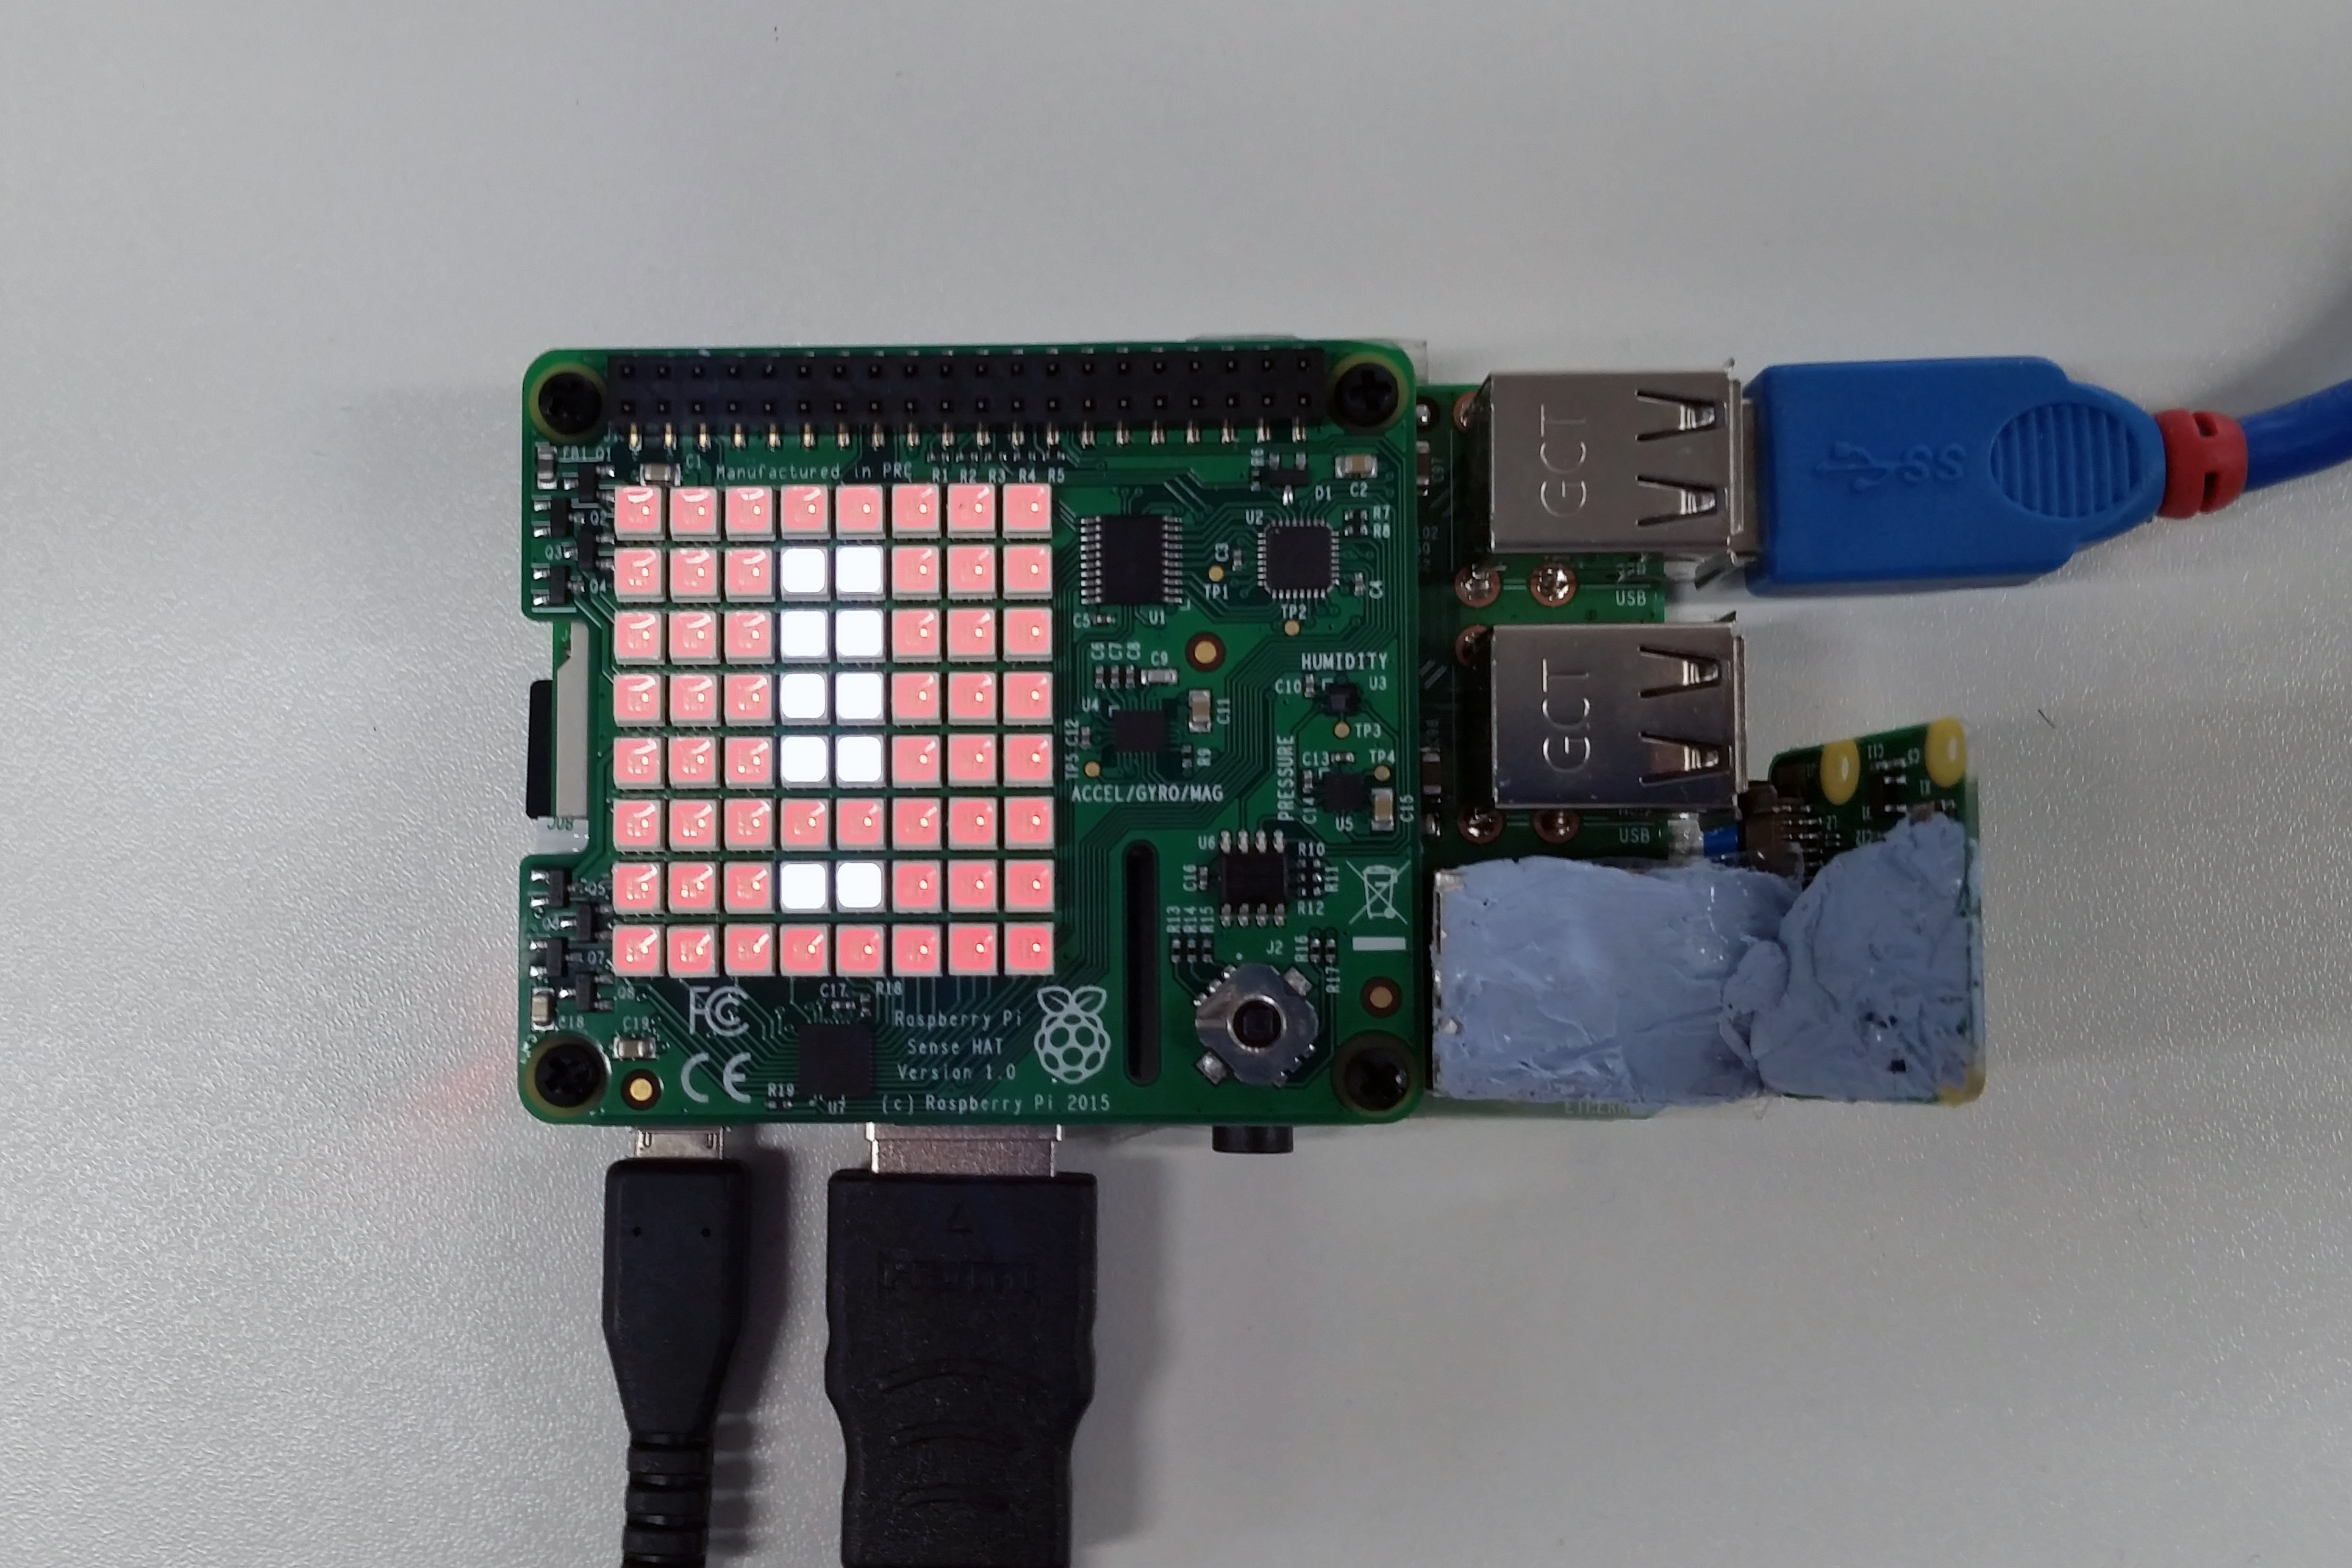
\includegraphics[width=0.305\textwidth]{errorpicture}\\
\end{tabular}
\caption{LED Matrix Status Photos}
\label{fig:led-matrix-status-photos}
\end{table}

Additionally, by pressing down on the joystick a user could either safely shut down the Raspberry Pi or reboot it. This functionality was added to help protect the integrity of the file system from unexpected power loss. As the device is designed to function automatically and without user interaction once powered, it is unlikely to have a keyboard or screen attached. Therefore, the user needs a simple method to quickly power off the device. Without such functionality, the user would likely simply remove power to the device, which has the potential of corrupting and destroying the file system, rendering the device unbootable until re-flashed.

\subsection{Automatically Running on Boot}

What is the point of a daemon script that doesn't run on boot? Nothing. That's why \lstinline{daemon.py}, OpenVPN, and either OpenMTC or OM2M (Depending on the build) are configured to run automatically on boot. This is achieved by proper configuration, and by using Linux \lstinline{/etc/init.d} scripts. Once installed, these scripts provide \lstinline{restart}, \lstinline{start}, \lstinline{status}, and \lstinline{stop} actions. Below is an example header:\\

\begin{lstlisting}[caption={init.d Header}, label={lst:header}]
#!/bin/sh
### BEGIN INIT INFO
# Provides:          SERVICE-NAME
# Required-Start:    $remote_fs $syslog
# Required-Stop:     $remote_fs $syslog
# Default-Start:     2 3 4 5
# Default-Stop:      0 1 6
# Short-Description: Start daemon at boot time
# Description:       Enable service provided by daemon.
### END INIT INFO

...
\end{lstlisting}

By adjusting the header, the name, description, order, and dependencies of a service can all be chosen. It is a flexible format, and what cannot be done in the header, can be done in the Bash script.

\subsubsection{Installing an init.d script}

\begin{enumerate}
\item Create a \lstinline{init.d} script from a template in \lstinline{/etc/init.d}.
\item Mark it executable with \lstinline{chmod +x /etc/init.d/$SERVICE-NAME}.
\item Install the init script with \lstinline{sudo update-rc.d $SERVICE-NAME defaults && sudo update-rc.d $SERVICE-NAME enable}.
\item Reboot the system, and service will run automatically.
\end{enumerate}

\subsection{Automatically Starting OpenVPN}

By default, OpenVPN will not automatically start, and will require the user to manually configure it after every boot. This can be fixed with the following two commands, assuming that \lstinline{config.ovpn} and \lstinline{certificate.crt} exist in the current directory.\\

\begin{lstlisting}[caption={Configuring OpenVPN}, label={lst:configuring-openvpn}]
sed -i -r 's/#AUTOSTART="all"/AUTOSTART="all"/g' /etc/default/openvpn
openvpn --client --config config.ovpn --daemon
\end{lstlisting}

The first line uncomments the \lstinline{AUTOSTART} variable in \lstinline{/etc/default/openvpn} so that when OpenVPN is started as a daemon (Runs in the background), on next boot it will start automatically.

\subsection{Building an image}

Once the Raspberry Pi was considered good and fully functional, an image was made. This was done by shutting down the Raspberry Pi to avoid damaging the file system, removing the microSD card, and inserting it into a computer to be read. Then, the device is mounted, and backed up using the following command:\\

\begin{lstlisting}[caption={Creating an image}, label={lst:backup}]
dd if=/dev/sdX conv=sync,noerror bs=64K | gzip -c > backup.img.gz
\end{lstlisting}

Then, to write the image to additional microSD cards, use the following command:\\

\begin{lstlisting}[caption={Restoring an image}, label={lst:restore}]
gunzip -c backup.img.gz | dd of=/dev/sdX
\end{lstlisting}

Now either the image, or microSD cards can now be shared. Due to how \lstinline{dd} creates disk images, images can only be flashed onto microSD cards with at least as much storage as the original microSD card. To resolve this issue, disk images can be shrunk using \lstinline{parted} or GParted.

\clearpage

  \chapter{Implementation}

The following section discuses Web Services, the different plug-ins, and how the product was federated with oneTRANSPORT.

\section{Web Services}
\label{sec:web-services}

The web server (NGINX) was split into different server blocks using virtual host configuration to make a more efficient use of resources. 

There are three server blocks:

\begin{itemize}
  \item Video Streaming Website (portal.sensivision.co)
  \item OM2M User Interface and Web API (om2m.sensivision.co)
  \item OpenMTC Web API (openmtc.sensivision.co)
\end{itemize}

\subsection{VPN}

As mentioned in the design section a VPN was added between the Raspberry Pi and cloud server. Following the tutorial\footnote{https://digitalocean.com/community/tutorials/how-to-set-up-an-openvpn-server-on-ubuntu-16-04} offered by Digital Ocean on setting up OpenVPN on server and client, the team produced the following set-up:

\begin{itemize}
\item \textbf{VPN Server}: 10.8.0.1
\item \textbf{Raspberry Pi 1 IP}: 10.8.0.6
\item \textbf{Raspberry Pi 2 IP}: 10.8.0.12
\end{itemize}

\section{OM2M Sensivision Plug-in}

The \lstinline{om2m.sensivision} plug-in was developed for interacting with the raspberry pi sensors on the MN-CSE and pushing the data to the IN-CSE. It was built based upon the om2m sample light plug-in described in section \ref{light plugin}.

The Sensivision plug-in was created for monitoring each sensor on a Sense HAT add-on board, whether through streams or individual readings.

\subsection{How it Works}

The \lstinline{Activator} class in each plug-in is it’s start point. Inside the class it has the \lstinline{public void start(BundleContext context) throws Exception} method which is called each time a plug-in starts up.

It first registers an IPE Service which, in this case, creates an interface from the Raspberry Pi to the oneM2M standard. The next step then involves ‘discovering’ any CSEs which may be connected to the Raspberry Pi. A CSE is an entity which represents a set of functions of which other entities (AEs, CSEs) can call e.g. Data Management, Device Management, M2M Service Subscription Management etc. The IPE uses the CSE to send requests and the CSE (when it receives a request from a third-party) uses the IPE to carry out the request.

\begin{figure}[H]
  \centering
  \includegraphics[width=\textwidth]{csemodel.png}
  \caption[OM2M IPE Architecture]{OM2M IPE Architecture \cite{om2mipesample}}
  \label{fig:IPEModel}
\end{figure}

From here, the \lstinline{start} method in the \lstinline{LifeCycleManager} class is called, which creates the application entity representing the Raspberry Pi and within AEs are created representing individual sensors. The AEs representing each sensor have containers within them which can be used to call any of the following 3 methods: \lstinline{GET}, \lstinline{START_STREAM} and \lstinline{END_STREAM}. 

As these containers are created on the MN, containers on the IN are also created to hold the data for each sensor. These containers have a fixed size so when the container becomes full and wants to add another content instance, it removes the oldest and adds the latest (comparable to enqueuing and dequeuing in the queue data structure rather than popping and pushing in a stack). 

The plug-in creates the AEs, containers and content instances is by the \lstinline{RequestSender} class. The sole use of the class is the \lstinline{createResource} method (other methods within the class call the \lstinline{createResource} method and are used for specific type of resources). The method creates a \lstinline{RequestPrimitive} instance (part of the OM2M’s common resource package). Using this instance, it sets multiple variables including the operation type (e.g. create for the creation of the AEs, containers and content instances) using enums, static fields, and additional arguments (the target ID, the resource). This creates the AE on the server once it uses the CSE from the controller to \lstinline{doRequest} passing the \lstinline{RequestPrimitive} as an argument.

The \lstinline{createResource} method returns a \lstinline{ResponsePrimitive} object. With the response the \lstinline{LifeCycleManager} gets the location of where it was created. It uses this as an argument for the IDs of the \lstinline{Descriptor} containers it next creates as well as logging the response from these creations. It then finally creates a content instance in the container. 

The plug-in receives requests via the \lstinline{Router} class. This is set up in the Activator class where it registers the \lstinline{IpeService}. It receives a \lstinline{RequestPrimitive} object from a CSE and from here the router class goes through various validation checks to ensure the request is valid. 

The request is checked for the operation query keyword defined in the \lstinline{SensorConstants} class, its corresponding value will match to one of the following (\lstinline{GET}, \lstinline{START_STREAM} and \lstinline{END_STREAM}). It then checks for the sensor identifier using the sensor query keyword, its corresponding value will match to one of the sensor names also defined in the \lstinline{SensorConstants} class. Using both values, it carries the request. It then returns a \lstinline{ResponsePrimitive}, setting the result of the operation as the content, the content-type a \lstinline{MimeMediaType.OBIX} (XML) and an \lstinline{ResponseStatusCode.OK} response status code.

\subsection{Operations}

Where the Sensivision plug-in differs greatly from the sample lamp plug-in is in the operations it can carry out. It can perform three of the following operations: \lstinline{GET}, \lstinline{START_STREAM} and \lstinline{END_STREAM}. 

All of these operations are managed by the \lstinline{ProcessManager} class whilst the operations themselves are represented by the \lstinline{ProcessRunner} class. The \lstinline{ProcessManager} is used when an operation should either be started or stopped. 

When a \lstinline{ProcessRunner} thread object is initialized it is given three arguments: commands to be executed (an array of Strings), the sensor data is to be collected from (String) and where the data is to be saved (String). The commands are carried out via Python script as there is a python library for retrieving data from a Sense HAT, all scripts differing slightly from one another. Once this object has been called to run, a \lstinline{ProcessBuilder} is used to create a \lstinline{Process} object. The input stream is taken from this object and from that a reader is created to read the incoming data. The data is saved by using the \lstinline{RequestSender} to send a content instance creation request to the IN to be created under the container corresponding to the sensor identifier in the IN.

\begin{itemize}
  \item \textbf{GET}\\
  Retrieve data once from a specified sensor and automatically saves data inside a data container. 
  \item \textbf{START\_STREAM}\\
  Start continuous stream of data from a specified sensor and automatically saves data inside a data container. \lstinline{GET} and \lstinline{START_STREAM} differ in only one extra command string: frequency. If the frequency is not given the \lstinline{Process} will only retrieve data once.
  \item \textbf{END\_STREAM}\\
  Terminates a stream for specified sensor, if one exists.
\end{itemize}

\subsection{OM2M Structure}

Structure of the system starts with the infrastructure node (shown in figure \ref{fig:OM2MInterface}), where all resources registered to it are accessible. Within the node, there is an RemoteCSE, which represents the middle node (labelled \lstinline{mn-pi} in figure \ref{fig:OM2MInterface} and point to the Raspberry Pi). 

\begin{figure}[H]
  \centering
  \frame{\includegraphics[width=1\linewidth]{om2minterface3.png}}
  \caption{OM2M IN Interface (1)}
  \label{fig:OM2MInterface}
\end{figure}

Figure \ref{fig:OM2MInterface2} shows the resources located under the remote CSE \lstinline{mn-pi}. These are the containers used for storing sensor data with the structure \lstinline{<sensor>_DATA}. This is all located on the IN server. The system was designed this way to avoid data storage on the light Raspberry Pi. 

There is a method whereby the middle node is directly accessible. From figure \ref{fig:OM2MInterface2}, this is the button located at the bottom right (labelled \lstinline{mn-pi-id}). When clicking this button, the IN redirects the user direly to the MN. 

\begin{figure}[H]
  \centering
  \frame{\includegraphics[width=1\linewidth]{INdata}}
  \caption{OM2M IN Interface (2)}
  \label{fig:OM2MInterface2}
\end{figure}

Inside the middle node (figure \ref{fig:OM2MInterface3}) there are multiple application entities, each of which represent a sensor containing the logic for querying and storing the data on the corresponding \lstinline{<sensor>_DATA} container on the IN. Each application entity has a container which has the content instances of the methods: \lstinline{GET}, \lstinline{START_STREAM}, and \lstinline{END_STREAM} shown in red on figure \ref{fig:OM2MInterface4}.

\begin{figure}[H]
  \centering
  \frame{\includegraphics[width=1\linewidth]{om2minterface4}}
  \caption{OM2M IN Interface (3)}
  \label{fig:OM2MInterface3}
\end{figure}

\begin{figure}[H]
  \centering
  \frame{\includegraphics[width=1\linewidth]{om2minterface5}}
  \caption{OM2M IN Interface (4)}
  \label{fig:OM2MInterface4}
\end{figure}

\section{OpenMTC Application}

Due to previously mentioned reasons, the code was ported from OM2M to OpenMTC to allow for further research, and ease of development.

\subsection{Creating Application Entities, Containers and Content}

Application entities are created by passing in the name of the entity to be created (in this case sensor\_data) and the location:\\

\begin{lstlisting}[caption={Creating Application Entities}, label={lst:creating-ae}]
location: '~/in-cse-1/oneM2M'
create_application(AE(resourceName='sensor_data'), location);
\end{lstlisting}

The containers were created by passing in information including the path where the container should be created (inside the application entity) and a container object containing information about the container such as the name (e.g. temperature) and number of content instances that the container can hold (in this case, ten was chosen).\\

\begin{lstlisting}[caption={Creating Containers}, label={lst:creating-containers}]
location = inside the previously created application entity
cont = Container(resourceName='temperature', max=10);
temperature_container = create_container(location, cont); 
\end{lstlisting}

The containers were stored in the Python script as a mapping of the resource name of the container to the container instance, allowing easy access for operations such as adding content instances.\\

\begin{lstlisting}[caption={Creating Content Instances}, label={lst:creating-content-instances}]
registered_sensors['temperature'] = temperature_container;
\end{lstlisting}

To add a content instance to a container, the container to add the data to and the data to add to it, in the form of a JSON, is needed. The JSON contains the current time stamp as well as the value to add (e.g. the current temperature for the temperature sensor). The corresponding container is retrieved via the container mapping described previously.\\

\begin{lstlisting}[caption={Creating Content}, label={lst:creating-content}]
sensor = 'temperature';
data = {
  'timestamp': time.time(),
  'value': value
}
push_content(registered_sensors[sensor], data);
\end{lstlisting}

\subsection{Running the Application}

To run, download the OpenMTC SDK \cite{OpenMTC2017OpenMTC}. Inside the \lstinline{openmtc-gevent} directory there is the \lstinline{run-backend} file and the \lstinline{run-gateway} file. The \lstinline{run-backend} file should be started, followed by the \lstinline{run-gateway}. The IPE created, as described in the previous section, is finally started.

\subsection{Structure}
\label{fig:Structure}

\begin{figure}[H]
\centering
\includegraphics[width=0.5\linewidth]{Type2DataZoom.png}
\caption{Type 2 Data}
\label{fig:Type2Data}
\end{figure}
  
Figure \ref{fig:Type2Data} shows the sensor data application entity created. Line 10 shows the type (type 2 is application entity) and line 11 shows the resource name (sensor\textunderscore data).\\

\begin{figure}[H]
\centering
\includegraphics[width=0.5\linewidth]{Type3DataZoom.png}
\caption{Type 3 Data}
\label{fig:Type3Data}
\end{figure}

Figure \ref{fig:Type3Data} shows the containers created. There is both a temperature and camera container of type 3 (representing containers).\\

\begin{figure}[H]
\centering
\includegraphics[width=0.5\linewidth]{Type4DataZoom.png}
\caption{Type 4 Data}
\label{fig:Type4Data}
\end{figure}

Figure \ref{fig:Type4Data} shows the inside of the temperature container. Content instances are of type 4 and there are a multitude of type 4 content instances within the temperature container.

\subsection{Rolling Database}

When the maximum number of content instances for a container has been reached, the oldest content instance is removed to make space for the new one. This done so the maximum size of a container may remain fixed and is known as a rolling database. To illustrate this easily, the \lstinline{temperature} containers maximum number of instances will be set to three and the values added will be in the form of strings.

Four content instances, containing the values \lstinline{1}, \lstinline{2}, \lstinline{3}, \lstinline{4}, were pushed into the container of size 3, in that order; what is expected to the see in the temperature container are three content instances where the oldest content instance has the value \lstinline{2}, the second oldest has the value \lstinline{3} and the most recent has the value \lstinline{4}.\\

\begin{lstlisting}[caption={Demonstrating a rolling database}, label={lst:rolling-database-demo}]
push_content(temperature_container, '1');
push_content(temperature_container, '2');
push_content(temperature_container, '3');
push_content(temperature_container, '4');
\end{lstlisting}

\begin{figure}[H]
  \centering
  \includegraphics[width=.5\linewidth]{3ContentInstancesZoom.png}
  \caption{Content Instances Inside Temperature Container}
  \label{fig:3ContentInstances}
\end{figure}

There are indeed three content instances inside the temperature container as shown by figure \ref{fig:3ContentInstances} (cin1, cin2 and cin3). To confirm the rolling database, \lstinline{cin1} must contain the value \lstinline{2}, \lstinline{cin2} must contain the value \lstinline{2} and \lstinline{cin3} must contain the value \lstinline{4}.

\subsection{Rolling Database Illustration}
\label{fig:RollingDatabase}

\begin{figure}[H]
\centering
\includegraphics[width=0.5\linewidth]{ContentInstance1Zoom.png}
\caption{Oldest Content Instance}
\label{fig:OldestContentInstance}
\end{figure}

\begin{figure}[H]
\centering
\includegraphics[width=0.5\linewidth]{ContentInstance2Zoom.png}
\caption{Second Content Instance}
\label{fig:SecondContentInstance}
\end{figure}

\begin{figure}[H]
\centering
\includegraphics[width=0.5\linewidth]{ContentInstance3Zoom.png}
\caption{Most Recent Content Instance}
\label{fig:MostRecentContentInstance}
\end{figure}

As shown by figure \ref{fig:RollingDatabase}, the values in the content instances (shown by 'con' on line 14) are exactly as predicted. 

\subsection{Camera Streaming}

The following was the process taken to stream the camera data:\\

\begin{lstlisting}[caption={Camera streaming pseudo code}, label={lst:camera-streaming-pseudo-code}]
Repeat until satisfied:
	Capture the current image frame
	Encode in base64 format
	Push data to the server
\end{lstlisting}

Initially camera streaming was done using Eclipse OM2M. This had a terrible frame rate, as a lot of time was required to parse the python code. It was limited to a couple of frames per second at a low 240p resolution. This was improved upon this by disabling logging and reducing the video quality. While it helped, it was not as much as expected. Fortunately, at this point in the project OpenMTC had just been open sourced.

Moving to OpenMTC improved the frame rate. It moved from a few frames per second to close to \textbf{20 frames per second} with a resolution of \textbf{300 $\times$ 300}. This made the stream not only usable but useful, properly demonstrating the powers of OpenMTC. Then, by adjusting JPEG quality, the resolution was raised to 720p, without any major impact on framerate. This proves that oneM2M is can transmit high resolution video, at a good framerate.

\section{Federation}

\subsection{Registering RemoteCSE}
\label{sec:remotecse}

The registration of RemoteCSEs procedures was used by IN-CSE to share data across INs. A successfully registered RemoteCSE is a one-way procedure giving the IN-CSE the ability to use the functions and services hosted on the remote CSE and access the data. This is federation in action.

\begin{figure}[H]
  \centering
  \includegraphics[width=\textwidth]{remotecse}
  \caption[RemoteCSE Registration Procedure]{RemoteCSE registration procedure}
  \label{remotecse}
\end{figure}
  
RemoteCSE registration is done through a single POST request specifying the type of resource to create (type 16). The CSE function take care of establishing communication with the specified host, verifying compatibility and exchanging information. Once this is completed, the IN-CSE with \lstinline{in-cse-id2} has a RemoteCSE resource in its structure named \lstinline{in-cse1} under the root. This will give access to the resources located on \lstinline{in-cse-id}, including the MN-CSE Raspberry Pi with sensor data represented by the \lstinline{mn-pi-id}. 

\subsection{OM2M and OpenMTC Federation}
\label{sec:federation}

The procedure described in section \ref{sec:remotecse} was used to achieve federation between OM2M and OpenMTC. CSE function located on OM2M can access resources in OpenMTC.

The XML shown in figure \ref{fig:federation-post-request} was sent as a HTTP POST request to the OM2M IN.

The fields mentioned in the XML are:

\begin{itemize}
\item \textbf{CSR}: Type of action Create RemoteCSE.
\item \textbf{RN}: Resource name to be displayed by OM2M. 
\item \textbf{POA}: Point of Access of the OpenMTC IN.
\item \textbf{CB}: Callback of the OM2M service provider.
\item \textbf{CSI}: CSE-ID of the OpenMTC IN.
\end{itemize}

\begin{figure}[H]
  \centering
  \includegraphics[width=\textwidth]{xml}
  \caption{Federation POST Request}
  \label{fig:federation-post-request}
\end{figure}

This created the remote CSE resource OpenMTC under the root on the OM2M IN that is visible on figure \ref{fig:cseopemtc} highlighted in red.

\begin{figure}[H]
  \centering
  \frame{\includegraphics[width=\textwidth]{om2mremotecse}}
  \caption[OpenMTC IN RemoteCSE register on OM2M]{OpenMTC IN RemoteCSE register on OM2M}
  \label{fig:cseopemtc}
\end{figure}

For OM2M's IN to access resources from OpenMTC's IN, the HTTP GET request shown in figure \ref{fig:fed} was sent to the OM2M server. The response, also shown in figure \ref{fig:fed}, displays the resource structure from the OpenMTC IN-CSE.  

\begin{figure}[H]
  \centering
  \includegraphics[scale=1]{fed}
  \caption[Federation OM2M to OpenMTC]{Federation OM2M to OpenMTC}
  \label{fig:fed}
\end{figure}

When attempting federating in the opposite direction (OpenMTC to OM2M) the following error appears in the OpenMTC console indicating the unsuccessful communication attempt:\\

\begin{lstlisting}[caption={Failed federation error}, label={lst:federation-error}]
ValueError: 28 is not a valid ResourceType
\end{lstlisting}

The reason for this error will be explained in the evaluation chapter of this report.
       
\subsection{oneTRANSPORT Federation}

The process of demonstrating federation with oneTRANSPORT: 

\begin{itemize}
  \item Run OM2M and OpenMTC IN-CSEs registered to the Raspberry Pi MN-CSEs available publicly. 
  \item Share the Point of Access (PoA) of the infrastructure to the client over email.
  \item The client would attempt the registration of the IN-CSEs through the RemoteCSE procedure, described in section \ref{sec:remotecse}, to try and gain access to the data.
  \item They would reply to the team via email with their findings and issues.
\end{itemize}

The Email Log in the Appendix B - OneTRANSPORT Federation Confirmation shows that the client managed to gain access to the OpenMTC IN-CSE and had access to the content instances in which video stream data was located. 

\clearpage

  \chapter{Testing}

Testing is crucial to verifying software. The team decided to take a multi-pronged approach towards testing, focusing on client feedback, visual testing, and code testing. By splitting up testing in such a manner, testing is done both informally and formally, covering the entire system from the ground up. Client feedback is crucial, and it is here that this section will start.

\section{Client Feedback}

Ultimately, client feedback is the most significant metric of success. Completing this project would be meaningless if it went against the clients wishes. Because of this approach, the team kept the client in the loop, ensuring that the team never deviated far from the client's desires. Table \ref{stats} quantifies interactions with the client. Throughout the project, the team revived feedback from the client, both good and bad, with changes made to keep the project on the right track.

\begin{table}[H]
\centering
\begin{tabular}{|l|l|}
\hline
\textbf{Number of Skype meetings}        & 4  \\ \hline
\textbf{Number of face to face meetings} & 1  \\ \hline
\textbf{Number of emails exchanged}      & 57 \\ \hline
\end{tabular}
\caption{Client interaction statistics}
\label{stats}
\end{table}

Ultimately, the client was happy with the project and the progress made. They received a copy of final report, and all the code created in the course of the project. It was a pleasure working with the client, and the team wishes them future success with oneTRANSPORT and the oneM2M standard.

\section{Visual Testing}

The purpose of these tests was to show the client data federation, and video streaming capabilities in action. Many tools were used including platform integrated tools, third party applications or self-developed visual testing platforms. By using a wide variety of tools to test, correctness is checked on many levels, increasing the team's confidence in the final product.

\subsection{Eclipse OM2M}

\begin{figure}[H]
  \centering
  \frame{\includegraphics[width=.6\linewidth]{INdata}}
  \caption{Eclipse OM2M CSE Resource Tree}
  \label{fig:viewing-the-eclipse-resource-tree}
\end{figure}

Eclipse OM2M is packaged with an interactive resource tree visualiser, that runs on each device. This interface was used to first experiment with the sample lamp plug-in after installing it, and then to aid in forming an understanding of how the overall OM2M set-up functioned. Once the plug-in was developed and ready to test, it was compiled and copied to the Raspberry Pi. However, the MN configuration files had to be altered before it could be properly run.

Initially, it did not fully work, so by using the interface the team began testing and narrowing down bugs. After some time, the plug-in was feature complete, with each feature fully tested and verified working.

This interface, while not crucial, was very helpful in development as it significantly simplified the development process. Without it, the team would have needed to research and use a third-part oneM2M client, or resort to a REST API client, and OM2M exposes and extends a powerful RESTful API. For example, if a method to create an AE was not working correctly, it would be absent from the interface and if the server's ID was changed, it would be shown in the interface under CSI.

\subsection{OpenMTC}

Unlike Eclipse OM2M, OpenMTC does not provide a native resource tree visualiser, and only serves a RESTful API. If the team had started off using OpenMTC instead of OM2M, it would likely have been necessary to research and use a third-party client. However, by this stage of the project, the team had formed a good understanding of how oneM2M functioned, and how to use it. As a result, the RESTful API was sufficient for testing and validating OpenMTC.

\begin{figure}[H]
  \centering
  \frame{\includegraphics[width=.6\linewidth]{insomnia}}
  \caption{The Insomnia REST client}
  \label{fig:insomnia-rest-client}
\end{figure}

Now to verify the plug-in, a third-party REST client by the name of Insomnia was used to create and run queries to verify the resources and data containing inside the OpenMTC system. Using Insomnia, each sensor was checked in turn and validated, checking streaming worked as expected. Overall this was a success, with the Python OpenMTC having significantly higher performance than Java OM2M. This could be due to either the overhead of the Java Virtual Machine being much greater than the Python runtime environment, and better software engineering.

\subsection{Video Streaming}

To measure the relative performance of the camera streams in both OM2M and OpenMTC, a visualization web application was developed. This web application consisted of two major parts:

\begin{itemize}
\item A PHP based oneM2M Proxy that would retrieve the last video frame on the client's behalf. This is necessary as JavaScript only supports relatively few protocols, and oneM2M is unfortunately not one of them.
\item A web page served by NGINX with JavaScript to poll for the latest frame, decode the base64 into a JPEG image, and display it to the client, with CSS to make the web page look professional.
\item While not technically part of the system, a modern web browser was used to view the web page.
\end{itemize}

This web application was publicly hosted in the Digital Ocean droplet, and then shared with the client. The different platforms were demonstrated and compared to identify the best performing solution. Ultimately while OM2M could broadcast roughly 5 frames per second, OpenMTC could broadcast roughly 20 frames per second with this set-up.

\section{Code Testing}

While visual testing is important, code testing is of at least equal importance. This section will describe the methods used.

\subsection{Pair Programming}

In critical sections of the project, pair programming was used to help quickly and safely develop the product with the insight of multiple team members. This was very useful as it allowed the team to discuss approaches and arrive at the correct one with less trial and error.

However, as the project progressed past such critical sections, pair programming was discontinued in favour of individual work, as it would have produced diminishing returns.

\subsection{Integration Testing}

To test the system as one, integration tests were written to validate the platform. The tests were split into 7 steps:

\begin{enumerate}
\item Login and retrieve the list of CSEs.
\item Find the CSI for \lstinline{mn-pi}.
\item Enumerate AEs, checking that every AE is registered.
\end{enumerate}

Now, the next four steps are repeated for each AE.

\begin{enumerate}
\setcounter{enumi}{4}
\item Retrieve the AE descriptor.
\item Retrieve the content instance.
\item Extract a list of actions.
\item Get a single value.
\end{enumerate}

Streams were not tested in this manner as unit testing covers the Python scripts themselves, and the difference between single values and streams in the plug-in is a couple of lines of code. 

\subsection{Unit Testing}

Unit tests were developed for the Python scripts to ensure that they each functioned correctly, and streamed data. During development, they were run on a Windows computer running Cygwin, and once finished they were then run on the Raspberry Pi itself. The full logs, sans stack traces, can be found in Appendix C for reference.

Running the tests on Windows results in about half of the available scripts functioning as intended, with nine running correctly. Considering that the Python scripts were intended to run on a Raspbian-lite powered Raspberry Pi with Sense HAT, it is quite surprising how many of the scripts worked in the first place. Windows natively supports a tiny fraction of APIs required for Python scripts, and obviously has zero support for the Sense HAT.

Unsurprisingly, running the tests on the intended platform results in every test passing. This is not a surprise as the scripts were created to run on the Raspberry Pi and had each been successfully run manually before. It was good, however to verify that they worked in such an automated manner, and it is significantly easier to rerun automated unit tests than resorting to manual testing.

\subsection{Regression Testing}

Due to the nature of agile methodology, the client frequently provided feedback and the team appropriately responded to it. After every change made, the team verified that the system was still fully functional and working as should be. At the start of the project, this was done manually, but extensively. Once Unit testing  was in place, the test suite was simply run instead.

\subsection{Automated Builds using Bitbucket Pipelines}

Eclipse's OM2M Java platform uses the Apache Maven build automation tool linking all the dependencies and describing how the software should be built using XML structures. To ensure that every commit built, BitBucket Pipelines were used to automatically build each commit and notify on error. Overall, this was rather successful, with it catching several commits that simply failed to build.

However, this could not be easily adapted to cover OpenMTC as Python does not have a compilation step. Besides static analysis, the only way to verify that a Python script runs without error, is to run it. Fortunately, though, while it couldn't automatically be tested, Python is so much easier to edit, alter, and fix on the Raspberry Pi itself, it was basically a non-issue. Whereas an error with Java OM2M resulted in a lengthy rebuild process, an error in Python OpenMTC could be resolved by ending the process, resolving the error in \lstinline{vim}, and restarting the gateway.

In future, it would have been a good idea to not only add some form of pipelines for verification but building up an automated test suite of unit and integration tests. This was however deemed outside the scope of this project, and thus skipped. It is something that would be interesting and useful to include in future work.

These tests were primarily for the team to verify the correctness of the code written or modified to save time when porting it over to the raspberry pi running the MN-CSE. But for the client these tests were not useful. To satisfy the client, other tools were used.

\clearpage

  \chapter{Evaluation}

This section will investigate the project's findings, any issues encountered during the research and implementation, and the approaches taken to resolve them.

To start, OM2M and OpenMTC will be compared in terms of usability, development of AEs and issues experienced. These would be primarily the team's experiences with development. Then a discussion detailing findings and issues with camera streaming through the OM2M and OpenMTC. Finally, an evaluation on the approaches taken with federations between OpenMTC, OM2M and oneTRANSPORT.

\section{Eclipse OM2M Platform}

\subsection{Usability}

Development for OM2M applications requires a specific version of the Eclipse IDE only. Following the tutorial on installing all the necessary packages for development some of the team ran into OS issues with Windows 10 and had to use Linux Ubuntu 16.04 Desktop or Linux Mint Sylvia 18.3 Virtual Machines to get the development environment set-up. From the team's experience, it was almost impossible to know which OSs will support the required development environment and which will not, out of the box.

Packages used in OM2M were dependent on Java version 7 and would fail with Java version 8. Therefore, it was not possible to take advantage of the new technologies that Java 8 provides, such as the lambda expressions. Members of the team had to modify their Java Runtime Environment (JRE) during set-up as most members' environments had been set up to use a Java 1.8 (Java version 8) platform instead of a Java 1.7 (Java version 7) platform. 

\subsection{Coding}

The code given in the sample plug-in is relatively simple to understand, once the time had been taken. The encapsulation of it made it straightforward to alter it for the needs of the project \ref{om2mpluginstruct}. Although, when a portion of code went misunderstood, the team had to go through many pages of oneM2M documentation to figure out the misunderstanding. The same would be said for portions of written code the team made that did not behave in the way it was intended.

\begin{figure}[H]
  \centering
  \includegraphics[scale=1]{om2mpluginstructure}
  \caption{OM2M Plug-in Structure}
  \label{om2mpluginstruct}
\end{figure}

Eclipse OM2M does not provide specifications, but rather provides guides on implementing certain elements of the OM2M platform in a specific manner. The team had to resort to using these and documentation from the oneM2M site \cite{onem2mhome}.

Whilst the guides are useful, they do not provide all the information required to completely build a custom OM2M system. Although the technical documents on the site were useful for understanding the core concepts that drive oneM2M, each document was extremely large in length and took multiple reads to fully comprehend. On top of this there were slight nuances with how OM2M works in comparison to how oneM2M states certain elements should be implemented, because of this the team had to experiment with their methodologies until a solution was found.

\subsection{Interface}

As mentioned in the previous chapter, Eclipse OM2M provides a highly intuitive interface (an interactive resource tree visualiser). This interface allows administrators/users of the system to see what is going on in real time and to also interact with it. It is automatically run on OM2M start-up, so by simply navigating to the device in a web browser, users can quickly and easily browse the entire resource tree structure as well as make REST calls without using REST API clients (e.g. Postman or Insomnia) to create HTTP requests on the behalf of users.

The interface is static HTML served by a Jetty web server. Visualising and interactivity is not a result of server-side processes but is the result of JavaScript running client-side.

Due to the OSGi modular approach taking in creating OM2M, it is trivial to enable, disable, or remove such components. In future work, this would allow the team to remove the visualiser if deemed necessary.
 
\subsection{Maven \& Bitbucket Pipelines}

Maven's build and install command was useful to verify that the entire project will build before deploying it on the server and gateway. However, most failures occurred because of the aforementioned Java SE problem.

Bitbucket pipelines also allowed the team to verify whether a commit that was pushed broke the system. In the case of a pushed commit breaking the system, the whole team would be notified would remedy the situation hastily. Most of the time this would not happen as, a commit that breaks the system would not pass the Maven build tests. However, as some of the team occasionally failed to verify with Maven or used a separate IDE, the team was glad that Bitbucket acted as a secondary measure.

\section{OpenMTC Platform}

\subsection{Usability}

Application development for OpenMTC was more accessible than OM2M. Separate Python files were written and then were launched independently from IN and MN and attached to either of them. There was no need to compile or build the project, as it was written in Python (an interpreted language), it was possible to directly change the Python files from the Raspberry Pi, as opposed to OM2M where files were compiled on a separate computer and then copied over to the Raspberry Pi due to its low hardware capabilities.

OpenMTC does not provide a visual interface for managing and visualising the resource structure inside the IN or MN. It only opens a RESTful API. Therefore, a third-party REST API application such as Insomnia\footnote{REST API client https://insomnia.rest/} was required for querying the API.

With the experiences and skills of the team, it was estimated that the task of creating a resource visualisation web interface would not be complicated but this task was outside the scope of this project.

\subsection{HTTPS Issues}

The IN servers as well as InterDigital's oneTRANSPORT were using HTTPS as a communication mechanism. When trying to register an OpenMTC IN-CSE as a RemoteCSE on OM2Ms or oneTRANSPORT's IN-CSE, there were issues validating client SSL certificates from OpenMTC on the server. In an HTTPS communication instantiation, server verification of the client certificate is optional, but OpenMTC forced this check when using HTTPS. The code in figure \ref{https}\footnote{https://github.com/OpenMTC/OpenMTC/blob/d3f33aa1536e9c1039264d2b2f2045d776447745/common/openmtc-oneM2M/src/openmtc\_oneM2M/client/http.py\#L95-L110} shows the code responsible for establishing connection to an IN host via HTTP(S). 

\begin{figure}[H]
  \centering
  \includegraphics[width=.75\linewidth]{https}
  \caption{Source Code from OpenMTC}
  \label{https}
\end{figure}

To resolve this issue, modifications had to be made to the communication establishment between the client (IN-CSE) and server (other IN-CSE) and remove the parameter that passes the client certificate. Only the client would perform server certificate versification and the server would trust all clients connecting. 

In the figure \ref{https}, \lstinline{HTTPclient} called from an OpenMTC IN-CSE trying to establish a connection with another IN-CSE. Passed in to the function are parameters for locating the server (\lstinline{host} and \lstinline{port}) as well as \lstinline{ssl_options}. Part of the SSL options are the client certificates passed to the server. Server-side verification is an optional step and by removing this step a valid connection can be established. 

\section{Video Streaming Through oneM2M}

This section will evaluate the implementations of video streaming as well as giving information to the client about future work in this area.

\subsection{OM2M}

Disabling console logging for the MN-CSEs and IN-CSEs allowed the processing of image data to be faster, resulting in a higher frame rate at a higher quality. The stream was running at around 5 frames per second which resulted in the live video feed not being fluid.

Parsing the data image from Python to Java proved to be the main issue which resulted in the low frame rate of the stream. Although this simplified the development process for the team it effected the performance of the video stream

Java's virtual machine and heavy XML document structure was also an issue when interacting with the camera data.

Future work with OM2M to improve its effectiveness should ideally be on micro controllers with greater hardware capabilities, be only interacting with the Raspberry Pi through Java libraries and using a JSON structure for simplified parsing. 

\subsection{OpenMTC}

Compared to OM2M, video streaming using OpenMTC was much more successful. This was likely due to lower overheads of the Python runtime environment when compared to the Java Virtual Machine, and the simpler architecture of OpenMTC in general.

While OM2M managed to achieve 5 frames per second, OpenMTC could broadcast 20 frames per second. This is a significant improvement, it is the difference between a slide show, and somewhat fluid motion.

This was mainly due to the fact that the image data did not require any parsing between programming languages as OpenMTC and the Raspberry Pi scripts were all written in Python. OpenMTC uses the JSON structure for serialization which requires less processing and parsing then XML used by OM2M.    

\subsection{Live Video Feed Website}

The live video feed website was only made as a testing platform to visualize the data being sent other oneM2M system. It was not built with scalability or future usability in mind.

Every web client that opened the video feed using a browser would generate 20 requests a second to the In-CSE requesting the latest data from the video feed. For example, 10 clients would generate 200 requests per second that could lead to DDOS (Distributed Denial of Services) being performed on the public facing IN-CSE server.

If the client wants to reproduce this project, the team suggests taking advantage of the subscription and notification mechanisms implemented in most oneM2M platforms described in section \ref{sec:sub}.

The web server hosting the video feed would subscribe to the IN-CSE telling it to update when a new video frame is available. The IN-CSEs security services can authenticate and authorize the application requesting the subscription. Once an image frame is available it would notify the web server with the data that can be displayed to the user.

\section{oneM2M Platform Federation}

In the context of the implementation, the team did not achieve mutual federation between service providers. Between open source implementations (OM2M and OpenMTC), only one way federation was established due to the \lstinline{ValueError: 28 is not a valid ResourceType} error. With regards to oneTRANSPORT, data was federated while their platform required extra authentication that will be explained in this section.  

\subsection{OM2M and OpenMTC}

Both IN-CSEs from OM2M and OpenMTC have a list of Supported Resource Types (SRT) mentioned in listing \ref{lst:srt} OpenMTC's SRTs is subset of OM2Ms SRTs and as it can be seen in listing \ref{lst:srt}, OpenMTC is missing the resource type 28 for flexible containers. Therefore, a two-way federation was not possible due to the error \lstinline{ValueError: 28 is not a valid ResourceType}.\\

\begin{lstlisting}[caption={OM2M and OpenMTC supported resource types}, label={lst:srt}]
OM2M:    1 2 3 4 5 9 14 15 16 17 23 28
OepnMTC: 1 2 3 4 5 9 14 15 16 17 23
\end{lstlisting}

For mutual federation to occur, both IN servers must implement the exact same set of resource types (SRTs) otherwise only one-way federation will be possible.

\subsection{OpenMTC and oneTRANSPORT}

Because of oneTRANSPORTs security design, it required specific headers to be present in every request when communicating with its IN-CSE. This therefore required a modification in the underlying HTTP communication of the platform choice. Using OpenMTC it was easy to locate the section of the code that needed modification (figure \ref{headers}).

\begin{figure}[H]
  \centering
  \includegraphics[width=.93\linewidth]{headers}
  \caption{Header Injection Location in OpenMTC}
  \label{headers}
\end{figure}

When translating oneM2M requests to HTTP requests, the translator displayed in figure \ref{headers} could have the functionality for custom headers added so that oneTRANSPORT can authenticate and authorize  the IN used. 

This would only be necessary to access oneTRANSPORT data. But, because the OpenMTC IN-CSE did not implement any custom requests authentication, oneTRANSPORT could successfully query data without the previous changes.

\clearpage

  \chapter{Future Work}

As with any major research project, there is always more that can be done. It is rare that when researching one topic, no other relevant topics are found. This project was no exception, so in this section potential areas of future work will be discussed.


\section{Federation Mechanisms}
\label{sec:sub}

This project only use the RemoteCSE resource type to establish a connection between INs in order to inter exchange data. Although this was a valid approach, oneM2M also specifies a subscriptions resource type that can be applied for data federation. Subscriptions allow a one way exchange of data between two servers. \lstinline{Server A} will register a subscription to \lstinline{Server B} on a specific resource such as new content instances (representing the data). When a content instance is created on \lstinline{Server B} in the specified resource, \lstinline{Server A} will receive a notification request containing the new data.

While subscriptions would considerably reduce the network usage between the two servers (as \lstinline{server A} only send one HTTP request to \lstinline{Server B} for the initial subscription), it will require more custom AEs to be created with the task of listening for notifications and parsing them to the data store. The team will suggest investigating the use of subscriptions for federating data between INs and comparing them to RemoteCSEs. 

\section{Increasing Complexity}

The current system is relatively simple, consisting of a few Raspberry Pis, Sense HATs, Camera, Cloud Server, and oneTRANSPORT. Federation has been demonstrated, but only on a small scale.

It would be interesting to investigate how the project handles increasing complexity due to a larger number of connected gateways, federation between more servers, and larger amounts of data. Typically, IoT platforms are designed to be deployed in constrained environments in their thousands.

For example, it is suspected that the video streaming functionality is unlikely to handle significant scaling and would need to be adapted to cope.

\section{Investigating protocols such as CoAP and MQTT}

While this project only used HTTP, oneM2M is designed to work seamlessly across different protocols such as CoAP and MQTT. Each protocol has advantages and disadvantages, and picking one is simply the matter of balancing trade-offs.

HTTP is a older protocol originally designed for transmitting documents over the internet, forming the basis of the World Wide Web. It enjoys widespread adoption, is easily understood, and massively interoperable. However, for a constrained device, the overhead of HTTP and Transmission Control Protocol (TCP) may be too great.

CoAP, on the other-hand, is a lightweight protocol that allows a multitude of devices to communicate efficiently. An open standard, but with less support than HTTP. It is however designed to interoperate with the web, so the developer curve is lessened when compared with MQTT. It operates over the User Diagram Protocol (UDP), which is light weight when compared with TCP \cite{chen2014constrained}.

MQTT is an even simpler protocol. It is open, incredibly flexible, and acts as a binary pipe. This gives developers incredible control, but in turn requires significantly more development time. Like CoAP, it operates over UDP.

\section{Exploring New Environments}

This project has taken place in an environment with rich computing capabilities. It would be interesting to explore how to adapt this work to new, constrained environments. These environments could include environments that are simply more separated, to going off the grid on new hardware platforms.

For example, base stations away from civilisation, or drones used to collect real-time data on air pollution. The data collected would be very interesting.

\section{Video Streaming}

The current system for video streaming could use work, and there are two different approaches that could be taken.

\subsection{oneM2M for Advertising and Control}

While oneM2M is certainly capable of broadcasting video, this report proves that, it was not designed for such a task and there are other protocols out there that may be better suited for it. One option would be to use oneM2M to advertise, and control video broadcast over such protocols, instead of directly using oneM2M itself. This would combine the power of oneM2M with the efficiency of protocols designed for video streaming.

There are many different video broadcasting protocols, including, but not limited to: Real-Time Streaming Protocol (RTSP), Dynamic Adaptive Streaming over HTTP (MPEG-DASH), Microsoft Smooth Streaming (MSS), HTTP Dynamic Streaming (HDS), and HTTP Live Streaming (HLS). If low latency is required, look into using RTSP. If widespread client support is required, look into using MPEG-DASH or HLS.

However, as such a system bypasses most of oneM2M, federation would not supported out of the box, and would need to be re-engineered. Additionally, firewall and NAT issues would each need to be addressed in turn.

\subsection{Motion JPEG}

Currently, each client connects to the server and polls it for updates at a fixed interval. However, from testing it was found that this retrieval is not particularly quick and has formed a major bottleneck. Further improvements would require moving from the current system to creating a Motion JPEG proxy that connects and subscribes to the IN-CSE on the client’s behalf. 

This would change from a polling model to a subscription model (Which would be rather difficult to do with just JavaScript) and ultimately only have a single proxy connecting to oneM2M instead of each client. This would reduce system load, decrease latency, and generally improve the streaming experience all around. This is possible as a motion JPEG stream is quite literally a sequence of concatenated JPEG stills served via a connection that isn't closed by the server. And best of all, MJPEG is widely supported by all major browsers with a performant poly-fill available for Internet Explorer. 

\section{Dashboard Visualisation Integration with Grafana}

Originally, the team intended to create a dashboard to visualise the project using HTML5 technologies. However, after communicating with the client, it was decided that this would essentially be a waste of time. They had their own solution using a Graphite database and Grafana for visualisation. So therefore, the feature was scrapped in favour of focusing on more important aspects of the project.

As future work, this Graphite and Grafana system could be investigated and duplicated to gather a fuller understanding of how the entire system works. This could then be used to combine data from different implementations of the oneM2M standard (such as oneTRANSPORT) and visualise them in an intuitive manner, thereby creating a fully-fledged application.

\clearpage

  \chapter{Conclusion}

The aim of this project was to demonstrate the federation of different implementations of the oneM2M standard, specifically with InterDigital's proprietary platform, oneTRANSPORT. This was shown to be possible. Additionally, this project demonstrated the capabilities of the platform to support video streaming.

The team developed and deployed plug-ins for two open source platforms, OM2M and OpenMTC. These were deployed on local Raspberry Pis connected to real-time sensors and cloud hosted web servers for storage. The Raspberry Pi set-up provided the client with a compact, portable and multi-functional device used for gateways.

Video streaming over HTTP through oneM2M was proven to be feasible on the OpenMTC platform, which provided a stable 20 frames per second. However OM2M platform's heavy parsing only provided a maximum of 5 frames a second. Federation was completed on two fronts:

\begin{itemize}
\item \textbf{Between the two open source platforms OM2M and OpenMTC}. Resources and functions saved on the OpenMTC server were accessed by the OM2Ms IN server. Although bi-directional data exchange was not possible due to OpenMTC's unsupported resource type. 
\item \textbf{Between OneTRANSPORT and OpenMTC}. The client's oneTRANSPORT platform could access the real-time sensor data hosted on the OpenMTC's IN server. However, mutual data communication could not be established as a result of oneTRANSPORT using a custom authentication header. A solution was suggested into how OpenMTC can support custom HTTP headers. 
\end{itemize}

By demonstrating federation between private and public services providers, this report proves the viability of using platforms implementing the oneM2M standard. If more and more companies adopt the standard throughout the coming years, interoperability of many of systems will create a large network of interconnected devices. They will be able to communicate together, enriching IoT data that will help change the world.
% DAAAM what an ending 

\clearpage


  \setcounter{secnumdepth}{-1}
  \chapter*{References}
  \label{sec:references}
  \addcontentsline{toc}{chapter}{\nameref{sec:references}}
  \printbibliography[heading=none]
  \clearpage

  \chapter{Appendix}

Turn over for the appendices.

\clearpage

\section{Appendix A - Gantt Charts}

\begin{center}
\includegraphics[scale=0.31,angle=90]{gatt}
\end{center}

\section{Appendix B - Communications Log}

The group met with the client, InterDigital on a weekly basis. Due to the clients London location, most were conducted over Skype, however a few were face to face. Additionally, the client was kept in the development loop with frequent emails asking for design input and implementation feedback. The list of email conversations can be found below:

\subsection*{OneTRANSPORT Federation Confirmation}
\label{sec:fed-conf}

\begin{lstlisting}
Great.
 
I was able to retrieve the contents of your CSE from a version of our CSE running locally:
 
+ curl -s -H 'Accept: application/json' -H 'X-M2M-RI: discover-remotecse2' -H 'X-M2M-Origin: CsuperAE' 'http://localhost:9011/~/in-cse-id/main?fu=1'
{
  "m2m:uril": [
    "/in-cse-id/main",
    "/in-cse-id/main/acp_admin",
    "/in-cse-id/main/mn-pi",
    "/in-cse-id/main/mn-pi/accelerometer_DATA",
    "/in-cse-id/main/mn-pi/camera_DATA",
    "/in-cse-id/main/mn-pi/camera_DATA/cin_145974492",
    "/in-cse-id/main/mn-pi/camera_DATA/cin_148737069",
    "/in-cse-id/main/mn-pi/camera_DATA/cin_183274186",
    "/in-cse-id/main/mn-pi/camera_DATA/cin_267279449",
    "/in-cse-id/main/mn-pi/camera_DATA/cin_307899785",
    "/in-cse-id/main/mn-pi/camera_DATA/cin_831851713",
    "/in-cse-id/main/mn-pi/camera_DATA/cin_865024078",
    "/in-cse-id/main/mn-pi/camera_DATA/cin_909142608",
    "/in-cse-id/main/mn-pi/camera_DATA/cin_928272334",
    "/in-cse-id/main/mn-pi/camera_DATA/cin_985322460",
    "/in-cse-id/main/mn-pi/compass_DATA",
    "/in-cse-id/main/mn-pi/cpu_DATA",
    "/in-cse-id/main/mn-pi/disk_DATA",
    "/in-cse-id/main/mn-pi/gyroscope_DATA",
    "/in-cse-id/main/mn-pi/humidity_DATA",
    "/in-cse-id/main/mn-pi/memory_DATA",
    "/in-cse-id/main/mn-pi/null_DATA",
    "/in-cse-id/main/mn-pi/one_DATA",
    "/in-cse-id/main/mn-pi/orientation_DATA",
    "/in-cse-id/main/mn-pi/pressure_DATA",
    "/in-cse-id/main/mn-pi/process_DATA",
    "/in-cse-id/main/mn-pi/quality_DATA",
    "/in-cse-id/main/mn-pi/rand_DATA",
    "/in-cse-id/main/mn-pi/temperature_DATA",
    "/in-cse-id/main/mn-pi/time_DATA",
    "/in-cse-id/main/mn-pi/uptime_DATA",
    "/in-cse-id/main/mn-pi/wifi_DATA",
    "/in-cse-id/main/mn-pi/zero_DATA"
  ]
}
 
Are you able to briefly describe the different containers that I see listed? And how did the camera data get to the webpage?
 
Owen.
\end{lstlisting}

\subsection*{Full Email Log}

% This needs to be stripped on UTF8 characters such as fancy ..., ", and ' before it will compile
\begin{lstlisting}
13 conversations, 57 messages:

parchkov d. (dp1u12) <dp1u12@soton.ac.uk>GDP feedback
Hi Owen, As part of our report we would like to include feedback from yourself about what you learnt from this project. If possible could you please send it before Wednesday 31st of January. Kind Regards, Dennis Parchkov .
Tracy Melvin <tm@ecs.soton.ac.uk>Group Design Project, University of Southampton
Dear All Please find attached a scanned copy of the fully signed project agreement Apologies for the delay regards Tracy Melvin Optoelectronics Research Centre and Electronics and Computer Science University of Southampton, UK +44(0)2380596505
Griffin, Owen <Owen.Griffin@InterDigital.com>GDP documentation(2 messages)
OK. Thanks for letting me know. Good luck with your exams. ________________________________ From: parchkov d. (dp1u12) <dp1u12@soton.ac.uk> Sent: 10 January 2018 11:15:58 To: Griffin, Owen Cc: adademir a. (aa8g13); ipindamitan e. (ei1g14); pournazari dezfouli a. (apd1g14); consterdine m. (mc21g14)...
parchkov d. (dp1u12) <dp1u12@soton.ac.uk>GDP communication update(18 messages)
We'd prefer Wednesday early afternoon, could you do 1200 or 1300 ? Dennis Parchkov From: Griffin, Owen <Owen.Griffin@InterDigital.com> Sent: 11 December 2017 13:36:46 To: parchkov d. (dp1u12) Cc: adademir a. (aa8g13); consterdine m. (mc21g14); pournazari dezfouli a. (apd1g14); ipindamitan e. (e...
parchkov d. (dp1u12) <dp1u12@soton.ac.uk>OM2M camera streaming
Hi Owen, We've got a working demo of camera streaming through OM2M. Here is a link of the video feed: http://openmtc.sensivision.co/ We have set it to 20 frames a second at a resolution of 200x150 pixels, but as it can be seen it only can do 1.5 frames a second. We have also disabled all lo...
parchkov d. (dp1u12) <dp1u12@soton.ac.uk>GDP meeting
Hi, Thanks for the meeting today. Here are a couple of the links we mentioned today: - OpenMTC(https://github.com/OpenMTC/OpenMTC, http://www.open-mtc.org/) - Platforms inter working slides: (see attachment) To summarise the next steps: - Investigate the remoteCse registra...
Griffin, Owen <Owen.Griffin@InterDigital.com>GDP project update
________________________________ From: parchkov d. (dp1u12) Sent: 23 November 2017 17:49:14 To: parchkov d. (dp1u12); Mohammed El-Hajjar; Cepeda, Rafael Cc: adademir a. (aa8g13); ipindamitan e. (ei1g14); pournazari dezfouli a. (apd1g14); consterdine m. (mc21g14) Subject: Re: GDP project update ...
parchkov d. (dp1u12) <dp1u12@soton.ac.uk>GDP project update(5 messages)
Hi, Thanks Owen. Monday afternoon would be good for us, preferably some time between 12 and 2 or 4 to 5. But if you are busy we can arrange it outside those times. Let us know when you are free, Kind Regards, Dennis Parchkov From: Mohammed El-Hajjar <meh@ecs.soton.ac.uk> Sent: 23 Novem...
parchkov d. (dp1u12) <dp1u12@soton.ac.uk>GDP project progress(7 messages)
Hi Owen, Yes, we have received the camera. We are close to finishing up on the second sprint (data storage, om2m IN-cse communication and sensor streaming). Our presentation is due on Tuesday, we will send you the slides once it is done. We are keen to show you what we have produced. Kind Re...
parchkov d. (dp1u12) <dp1u12@soton.ac.uk>Project Progress(8 messages)
Hi, Wednesday 9:30 is perfect for us. Kind Regards, Dennis Parchkov _____________________________ From: Mohammed El-Hajjar <meh@ecs.soton.ac.uk> Sent: Friday, October 27, 2017 10:58 AM Subject: Re: Project Progress To: Cepeda, Rafael <rafael.cepeda@interdigital.com>, parchkov d. (dp1u12) <dp1u...
Griffin, Owen <Owen.Griffin@InterDigital.com>Server SSH(3 messages)
Hi, The permissions of the "soton" home folder were set incorrectly, by something at somepoint. The SSH daemon won't allow remote access if the permissions of the /home/soton /home/soton/.ssh and /home/soton/.ssh/authorized_keys are set incorrectly. You should be able to log-in now. Owen. [ci...
Griffin, Owen <Owen.Griffin@InterDigital.com>Multi-vendor IoT GDP project(2 messages)
Done. n.b. opening common port numbers will result in your server being targeting by people trying to expose known vulnerabilities in software. Ensure whatever process listens on these ports is using the latest version and that you update the machine regularly to receive the latest security patche...
Griffin, Owen <Owen.Griffin@InterDigital.com>Sensors(8 messages)
Sorry, I've only just collected this email. The VM has been started again. From: parchkov d. (dp1u12) [mailto:dp1u12@soton.ac.uk] Sent: 15 October 2017 17:43 To: Griffin, Owen <Owen.Griffin@InterDigital.com> Cc: Cepeda, Rafael <Rafael.Cepeda@InterDigital.com>; Mohammed El-Hajjar <meh@ecs.soton.ac....
\end{lstlisting}

\section{Appendix C - Python Script Unit Testing}

\subsection*{Running on Windows with Cygwin}

Standard Error was redirected to \lstinline{/dev/null} because the environment is missing crucial Linux commands, and the \lstinline{sense-hat} library. It does not affect the results.\\

\begin{lstlisting}
$ python3 test.py 2> /dev/null
 - FAILED disk produced invalid output:
FAILURE: disk
Success: one
Success: process
 - FAILED wifi call (exit code = 1)
 - FAILED wifi didn't stream.
FAILURE: wifi
 - FAILED accelerometer call (exit code = 1)
 - FAILED accelerometer didn't stream.
FAILURE: accelerometer
 - FAILED compass call (exit code = 1)
 - FAILED compass didn't stream.
FAILURE: compass
 - FAILED orientation call (exit code = 1)
 - FAILED orientation didn't stream.
FAILURE: orientation
 - FAILED quality call (exit code = 1)
 - FAILED quality didn't stream.
FAILURE: quality
 - FAILED temperature call (exit code = 1)
 - FAILED temperature didn't stream.
FAILURE: temperature
Success: zero
Success: cpu
 - FAILED gyroscope call (exit code = 1)
 - FAILED gyroscope didn't stream.
FAILURE: gyroscope
Success: memory
Success: rand
Success: time
 - FAILED camera call (exit code = 1)
 - FAILED camera didn't stream.
FAILURE: camera
 - FAILED humidity call (exit code = 1)
 - FAILED humidity didn't stream.
FAILURE: humidity
Success: null
 - FAILED pressure call (exit code = 1)
 - FAILED pressure didn't stream.
FAILURE: pressure
Success: uptime

***

9 / 20 succeeded.
\end{lstlisting}

\subsection*{Running on the Pi}

\begin{lstlisting}
$ python3 test.py
Success: disk
Success: one
Success: process
Success: wifi
Success: accelerometer
Success: compass
Success: orientation
Success: quality
Success: temperature
Success: zero
Success: cpu
Success: gyroscope
Success: memory
Success: rand
Success: time
Success: camera
Success: humidity
Success: null
Success: pressure
Success: uptime

***

20 / 20 succeeded.
\end{lstlisting}

\section{Appendix D - oneM2M Plug-in Integration Testing}

\begin{lstlisting}
$ python3 integration.py
GET '/~/in-cse-id?rcn=5&lvl=1'

/in-cse-id/csr-388561514 discovered.

GET '/~/in-cse-id/csr-388561514?rcn=5&lvl=1'

/mn-pi-id identified.

GET '/~/mn-pi-id?rcn=5&lvl=1'

accelerometer found.
camera found.
compass found.
cpu found.
disk found.
gyroscope found.
humidity found.
memory found.
null found.
orientation found.
one found.
pressure found.
process found.
quality found.
rand found.
temperature found.
time found.
uptime found.
wifi found.
zero found.

Everything found!

GET '/~/mn-pi-id/CAE667525045?rcn=5&lvl=1'
GET '/~/mn-pi-id/cnt-742314538?rcn=5&lvl=1'
GET '/~/mn-pi-id/cin-969682273?rcn=5&lvl=1'
GET '/~/mn-pi-id/mn-pi/accelerometer?op=get&amp;sensorid=accelerometer?rcn=5&lvl=1'
accelerometer validated!

GET '/~/mn-pi-id/CAE723285051?rcn=5&lvl=1'
GET '/~/mn-pi-id/cnt-994252396?rcn=5&lvl=1'
GET '/~/mn-pi-id/cin-491213893?rcn=5&lvl=1'
GET '/~/mn-pi-id/mn-pi/camera?op=get&amp;sensorid=camera?rcn=5&lvl=1'
camera validated!

GET '/~/mn-pi-id/CAE233442688?rcn=5&lvl=1'
GET '/~/mn-pi-id/cnt-233116302?rcn=5&lvl=1'
GET '/~/mn-pi-id/cin-28793551?rcn=5&lvl=1'
GET '/~/mn-pi-id/mn-pi/compass?op=get&amp;sensorid=compass?rcn=5&lvl=1'
compass validated!

GET '/~/mn-pi-id/CAE282164977?rcn=5&lvl=1'
GET '/~/mn-pi-id/cnt-591162585?rcn=5&lvl=1'
GET '/~/mn-pi-id/cin-431135428?rcn=5&lvl=1'
GET '/~/mn-pi-id/mn-pi/cpu?op=get&amp;sensorid=cpu?rcn=5&lvl=1'
cpu validated!

GET '/~/mn-pi-id/CAE942637379?rcn=5&lvl=1'
GET '/~/mn-pi-id/cnt-226118581?rcn=5&lvl=1'
GET '/~/mn-pi-id/cin-429044346?rcn=5&lvl=1'
GET '/~/mn-pi-id/mn-pi/disk?op=get&amp;sensorid=disk?rcn=5&lvl=1'
disk validated!

GET '/~/mn-pi-id/CAE904983583?rcn=5&lvl=1'
GET '/~/mn-pi-id/cnt-17674755?rcn=5&lvl=1'
GET '/~/mn-pi-id/cin-247437892?rcn=5&lvl=1'
GET '/~/mn-pi-id/mn-pi/gyroscope?op=get&amp;sensorid=gyroscope?rcn=5&lvl=1'
gyroscope validated!

GET '/~/mn-pi-id/CAE279945101?rcn=5&lvl=1'
GET '/~/mn-pi-id/cnt-41184056?rcn=5&lvl=1'
GET '/~/mn-pi-id/cin-685786383?rcn=5&lvl=1'
GET '/~/mn-pi-id/mn-pi/humidity?op=get&amp;sensorid=humidity?rcn=5&lvl=1'
humidity validated!

GET '/~/mn-pi-id/CAE252855933?rcn=5&lvl=1'
GET '/~/mn-pi-id/cnt-405922709?rcn=5&lvl=1'
GET '/~/mn-pi-id/cin-30407995?rcn=5&lvl=1'
GET '/~/mn-pi-id/mn-pi/memory?op=get&amp;sensorid=memory?rcn=5&lvl=1'
memory validated!

GET '/~/mn-pi-id/CAE431092629?rcn=5&lvl=1'
GET '/~/mn-pi-id/cnt-92333482?rcn=5&lvl=1'
GET '/~/mn-pi-id/cin-887510275?rcn=5&lvl=1'
GET '/~/mn-pi-id/mn-pi/null?op=get&amp;sensorid=null?rcn=5&lvl=1'
null validated!

GET '/~/mn-pi-id/CAE404519751?rcn=5&lvl=1'
GET '/~/mn-pi-id/cnt-928399438?rcn=5&lvl=1'
GET '/~/mn-pi-id/cin-118366981?rcn=5&lvl=1'
GET '/~/mn-pi-id/mn-pi/orientation?op=get&amp;sensorid=orientation?rcn=5&lvl=1'
orientation validated!

GET '/~/mn-pi-id/CAE42864371?rcn=5&lvl=1'
GET '/~/mn-pi-id/cnt-362293291?rcn=5&lvl=1'
GET '/~/mn-pi-id/cin-904859540?rcn=5&lvl=1'
GET '/~/mn-pi-id/mn-pi/one?op=get&amp;sensorid=one?rcn=5&lvl=1'
one validated!

GET '/~/mn-pi-id/CAE822258315?rcn=5&lvl=1'
GET '/~/mn-pi-id/cnt-233107406?rcn=5&lvl=1'
GET '/~/mn-pi-id/cin-89757949?rcn=5&lvl=1'
GET '/~/mn-pi-id/mn-pi/pressure?op=get&amp;sensorid=pressure?rcn=5&lvl=1'
pressure validated!

GET '/~/mn-pi-id/CAE405939079?rcn=5&lvl=1'
GET '/~/mn-pi-id/cnt-779525290?rcn=5&lvl=1'
GET '/~/mn-pi-id/cin-541128502?rcn=5&lvl=1'
GET '/~/mn-pi-id/mn-pi/process?op=get&amp;sensorid=process?rcn=5&lvl=1'
process validated!

GET '/~/mn-pi-id/CAE976567664?rcn=5&lvl=1'
GET '/~/mn-pi-id/cnt-167259850?rcn=5&lvl=1'
GET '/~/mn-pi-id/cin-587622615?rcn=5&lvl=1'
GET '/~/mn-pi-id/mn-pi/quality?op=get&amp;sensorid=quality?rcn=5&lvl=1'
quality validated!

GET '/~/mn-pi-id/CAE687368448?rcn=5&lvl=1'
GET '/~/mn-pi-id/cnt-582719030?rcn=5&lvl=1'
GET '/~/mn-pi-id/cin-771539675?rcn=5&lvl=1'
GET '/~/mn-pi-id/mn-pi/rand?op=get&amp;sensorid=rand?rcn=5&lvl=1'
rand validated!

GET '/~/mn-pi-id/CAE706206913?rcn=5&lvl=1'
GET '/~/mn-pi-id/cnt-799800719?rcn=5&lvl=1'
GET '/~/mn-pi-id/cin-602339587?rcn=5&lvl=1'
GET '/~/mn-pi-id/mn-pi/temperature?op=get&amp;sensorid=temperature?rcn=5&lvl=1'
temperature validated!

GET '/~/mn-pi-id/CAE674164292?rcn=5&lvl=1'
GET '/~/mn-pi-id/cnt-321842948?rcn=5&lvl=1'
GET '/~/mn-pi-id/cin-414219939?rcn=5&lvl=1'
GET '/~/mn-pi-id/mn-pi/time?op=get&amp;sensorid=time?rcn=5&lvl=1'
time validated!

GET '/~/mn-pi-id/CAE848868795?rcn=5&lvl=1'
GET '/~/mn-pi-id/cnt-787411008?rcn=5&lvl=1'
GET '/~/mn-pi-id/cin-143364143?rcn=5&lvl=1'
GET '/~/mn-pi-id/mn-pi/uptime?op=get&amp;sensorid=uptime?rcn=5&lvl=1'
uptime validated!

GET '/~/mn-pi-id/CAE813045617?rcn=5&lvl=1'
GET '/~/mn-pi-id/cnt-561582012?rcn=5&lvl=1'
GET '/~/mn-pi-id/cin-330155780?rcn=5&lvl=1'
GET '/~/mn-pi-id/mn-pi/wifi?op=get&amp;sensorid=wifi?rcn=5&lvl=1'
wifi validated!

GET '/~/mn-pi-id/CAE273995163?rcn=5&lvl=1'
GET '/~/mn-pi-id/cnt-279888773?rcn=5&lvl=1'
GET '/~/mn-pi-id/cin-896751456?rcn=5&lvl=1'
GET '/~/mn-pi-id/mn-pi/zero?op=get&amp;sensorid=zero?rcn=5&lvl=1'
zero validated!

***

Test Success!!!
\end{lstlisting}

\section{Appendix E - Bitbucket Graphs}

\begin{figure}[H]
  \centering
  \includegraphics[width=\textwidth]{git}
  \caption{Bitbucket Commit Graphs in the OM2M Repository}
  \label{bitbucket-commit-graphs}
\end{figure}

\begin{figure}[H]
  \centering
  \includegraphics[width=\textwidth]{bitbucket-commit-graphs-2}
  \caption{Bitbucket Commit Graphs in the HATs Repository}
  \label{bitbucket-commit-graphs-2}
\end{figure}

\section{Appendix F - Bitbucket Pipelines}

\begin{figure}[H]
  \centering
  \includegraphics[width=\textwidth]{pipelines}
  \caption{Bitbucket Pipelines}
  \label{bitbucket-pipelines}
\end{figure}

\section{Appendix G - Example of Successful Maven Build \& Install}

\begin{figure}[H]
  \centering
  \includegraphics[width=.9\linewidth]{om2mmavensuccess}
  \caption{Maven Build and Install Success}
  \label{maven}
\end{figure}

\section{Appendix H - List of Files in Code Archive}

\dirtree{%
.1 \lstinline{archive.zip}.
.2 \lstinline{readme.md}.
.2 \lstinline{bash}.
.3 \lstinline{gateway.sh}.
.3 \lstinline{sensivision-daemon}.
.3 \lstinline{sensivision-gateway}.
.3 \lstinline{sensivision-server}.
.3 \lstinline{server.sh}.
.2 \lstinline{icons}.
.3 \lstinline{ok.png}.
.3 \lstinline{spinner.png}.
.3 \lstinline{tick.png}.
.3 \lstinline{unknown.png}.
.3 \lstinline{warning_blue.png}.
.3 \lstinline{warning_orange.png}.
.3 \lstinline{warning_red.png}.
.3 \lstinline{warning_yellow.png}.
.3 \lstinline{upscaled}.
.4 \lstinline{ok.png}.
.4 \lstinline{unknown.png}.
.4 \lstinline{warning_red.png}.
.4 \lstinline{warning_yellow.png}.
.2 \lstinline{latex}.
.3 \lstinline{appendices.tex}.
.3 \lstinline{conclusion.tex}.
.3 \lstinline{design.tex}.
.3 \lstinline{ecsgdp.cls}.
.3 \lstinline{evaluation.tex}.
.3 \lstinline{future.tex}.
.3 \lstinline{implementation.tex}.
.3 \lstinline{intro.tex}.
.3 \lstinline{main.tex}.
.3 \lstinline{manual.bib}.
.3 \lstinline{mendeley.bib}.
.3 \lstinline{planning.tex}.
.3 \lstinline{research.tex}.
.3 \lstinline{testing.tex}.
.3 \lstinline{images}.
.4 \lstinline{3ContentInstancesZoom.png}.
.4 \lstinline{bitbucket-commit-graphs-2.png}.
.4 \lstinline{camera.jpg}.
.4 \lstinline{ContentInstance1Zoom.png}.
.4 \lstinline{ContentInstance2Zoom.png}.
.4 \lstinline{ContentInstance3Zoom.png}.
.4 \lstinline{csemodel.png}.
.4 \lstinline{data_storage.PNG}.
.4 \lstinline{errorpicture.jpg}.
.4 \lstinline{fed.png}.
.4 \lstinline{functional.PNG}.
.4 \lstinline{gatt.pdf}.
.4 \lstinline{git.png}.
.4 \lstinline{headers.PNG}.
.4 \lstinline{https.PNG}.
.4 \lstinline{INdata.PNG}.
.4 \lstinline{initial_design.PNG}.
.4 \lstinline{insomnia.PNG}.
.4 \lstinline{lamp.PNG}.
.4 \lstinline{lamps.png}.
.4 \lstinline{nat.PNG}.
.4 \lstinline{nodes.PNG}.
.4 \lstinline{ok.png}.
.4 \lstinline{okpicture.jpg}.
.4 \lstinline{om2minterface2.png}.
.4 \lstinline{om2minterface3.png}.
.4 \lstinline{om2minterface4.PNG}.
.4 \lstinline{om2minterface5.PNG}.
.4 \lstinline{om2mmavensuccess.png}.
.4 \lstinline{om2mpluginstructure.png}.
.4 \lstinline{om2mremotecse.PNG}.
.4 \lstinline{om2m_fed.PNG}.
.4 \lstinline{pi.jpg}.
.4 \lstinline{pipelines.png}.
.4 \lstinline{remotecse.PNG}.
.4 \lstinline{setup.jpg}.
.4 \lstinline{step1.PNG}.
.4 \lstinline{step2.PNG}.
.4 \lstinline{step3.PNG}.
.4 \lstinline{Type2DataZoom.png}.
.4 \lstinline{Type3DataZoom.png}.
.4 \lstinline{Type4DataZoom.png}.
.4 \lstinline{unknown.png}.
.4 \lstinline{unknownpicture.jpg}.
.4 \lstinline{warning_red.png}.
.4 \lstinline{xml.PNG}.
.2 \lstinline{om2m}.
.3 \lstinline{.classpath}.
.3 \lstinline{.gitignore}.
.3 \lstinline{.project}.
.3 \lstinline{build.properties}.
.3 \lstinline{pom.xml}.
.3 \lstinline{META-INF}.
.4 \lstinline{MANIFEST.MF}.
.3 \lstinline{src}.
.4 \lstinline{main}.
.5 \lstinline{java}.
.6 \lstinline{org}.
.7 \lstinline{eclipse}.
.8 \lstinline{om2m}.
.9 \lstinline{sensivision}.
.10 \lstinline{Activator.java}.
.10 \lstinline{RequestSender.java}.
.10 \lstinline{Router.java}.
.10 \lstinline{constants}.
.11 \lstinline{Operations.java}.
.11 \lstinline{SensorConstants.java}.
.10 \lstinline{controller}.
.11 \lstinline{Controller.java}.
.11 \lstinline{LifeCycleManager.java}.
.10 \lstinline{utils}.
.11 \lstinline{ObixUtil.java}.
.11 \lstinline{ProcessManager.java}.
.11 \lstinline{ProcessRunner.java}.
.3 \lstinline{target}.
.4 \lstinline{local-artifacts.properties}.
.4 \lstinline{MANIFEST.MF}.
.4 \lstinline{org.eclipse.om2m.sensivision-1.1.0-SNAPSHOT.jar}.
.4 \lstinline{p2artifacts.xml}.
.4 \lstinline{p2content.xml}.
.4 \lstinline{classes}.
.5 \lstinline{org}.
.6 \lstinline{eclipse}.
.7 \lstinline{om2m}.
.8 \lstinline{sensivision}.
.9 \lstinline{Activator$1$1.class}.
.9 \lstinline{Activator$1.class}.
.9 \lstinline{Activator.class}.
.9 \lstinline{RequestSender.class}.
.9 \lstinline{Router.class}.
.9 \lstinline{constants}.
.10 \lstinline{Operations.class}.
.10 \lstinline{SensorConstants.class}.
.9 \lstinline{controller}.
.10 \lstinline{Controller.class}.
.10 \lstinline{LifeCycleManager.class}.
.9 \lstinline{utils}.
.10 \lstinline{ObixUtil.class}.
.10 \lstinline{ProcessManager.class}.
.10 \lstinline{ProcessRunner.class}.
.4 \lstinline{generated-sources}.
.5 \lstinline{annotations}.
.4 \lstinline{maven-archiver}.
.5 \lstinline{pom.properties}.
.2 \lstinline{openmtc}.
.3 \lstinline{start.py}.
.2 \lstinline{python}.
.3 \lstinline{accelerometer.py}.
.3 \lstinline{blink.py}.
.3 \lstinline{clear.py}.
.3 \lstinline{compass.py}.
.3 \lstinline{cpu.py}.
.3 \lstinline{disk.py}.
.3 \lstinline{gyroscope.py}.
.3 \lstinline{humidity.py}.
.3 \lstinline{joystick.py}.
.3 \lstinline{lowlight.py}.
.3 \lstinline{memory.py}.
.3 \lstinline{orientation.py}.
.3 \lstinline{pixels.py}.
.3 \lstinline{pressure.py}.
.3 \lstinline{process.py}.
.3 \lstinline{quality.py}.
.3 \lstinline{rotation.py}.
.3 \lstinline{scroll.py}.
.3 \lstinline{temperature.py}.
.3 \lstinline{time.py}.
.3 \lstinline{wifi.py}.
.2 \lstinline{tests}.
.3 \lstinline{integration.py}.
.3 \lstinline{test.py}.
.2 \lstinline{video}.
.3 \lstinline{fetch.php}.
.3 \lstinline{index.html}.
}

\clearpage

\end{document}
